\documentclass[PHIL101-Textbook.tex]{subfiles}
\begin{document}

\part[Predicate Logic]{Predicate Logic\\Symbolisation}\label{part:pl}

\chapter{The Language of \pl}\label{ch:plBuildingBlocks}

\section{Decomposing Statements}

\begin{center}
  \href{https://youtu.be/ssmzb8OaxBA}
  {\XeTeXLinkBox{\qrcode[height=25mm]{https://youtu.be/ssmzb8OaxBA}}}
\end{center}

Consider the following argument:
\begin{earg}
\label{willard1}
\item[]Phoenix is a logician.
\item[] All logicians are kind.
\item[\therefore] Phoenix is kind.
\end{earg}

\noindent This argument is valid. To see this, take any situation in which Phoenix is a logician and all logicians are kind. We do not know whether there are other logicians in this case, but we know that Phoenix is one of them. We further know from the second premise that anyone who is a logician is someone who is kind. So it must be that Phoenix is kind. Therefore, the argument is valid, because every case in which the premises are true is a case in which the conclusion is also true.  

\logic{Logicians sometimes like to work with counterexamples to demonstrate that arguments are valid. Here's how this might go with the Phoenix argument: 
  \begin{quote}Imagine there were a counterexample, i.e., a case in which the premises are true but the conclusion is false. From the truth of the first premise and the falsity of the conclusion, this would be a case in which Phoenix is a logician that isn't kind. If that were so, we would have at least one logician who isn't kind, which would make the second premise false. So our case would fail to be a counterexample. Hence, there cannot be a counterexample to the argument. The argument is therefore valid.\end{quote}
\noindent Because the argument is quite simple, appealing to counterexamples might seem to you like an overkill. But remember this strategy when you face arguments in the wild and wonder if they are valid: assume there's a counterexample, i.e., a case in which the premises are true and the conclusion is false, and try to get a contradiction. 
}

\mathematics{Working with counterexamples can be very efficient in mathematics. For those of you who have to sit in mathematics exams and have to provide proofs, try the counterexample methodology: assume that there is a case in which conditions set out in the problem hold, but the result you've been asked to proved doesn't. Use this information to derive a contradiction. If you succeed, you know that the result follows \emph{validly} from the conditions of the problem, and so you have an efficient proof.}

Let's try now to symbolise it in \tfl, and see if we get the same diagnosis. We might use this symbolisation key:

\begin{ekey}
\item[L] Phoenix is a logician.
\item[A] All logicians are kind.
\item[F] Phoenix is kind.
\end{ekey}
And the argument itself becomes:

\begin{center}
\begin{tabular}{llll}
&Phoenix is a logician. && $L$\\
  & All logicians are kind. && $A$\\
 \therefore &  Phoenix is kind. & \therefore & $F$
\end{tabular}
\end{center}

\noindent This is \emph{invalid} in \tfl, as can be see with a valuation that assigns 1 to $L$ and $A$, and 0 to $F$. Something has gone wrong. We have a valid argument whose symbolisation tell us that it's invalid. What's going on? 

The problem is not that we have made a mistake while symbolising the argument. This is the best symbolisation we can give \emph{in} \tfl. The problem lies with \tfl\ itself. `All logicians are kind' is about two kinds of things: logicians and things that are kind. Our symbolisation in \tfl\ fails to make this distinction, so we lose the connection between Phoenix being a logician and Phoenix being kind. In other words, connectives do not allow us to decompose statements like `All logicians are kind' into simpler components. This is why we need a more powerful formal system. 

To symbolise arguments like the preceding one, we will have to develop a new logical language which will allow us to \emph{split the atom}. We will call this language \acrfull{pl}.
The details of \pl\ will be explained throughout this chapter, but here is the basic idea. First, we have \emph{names}. Names allow us to refer directly to things, like Phoenix. In \pl, we indicate names with lowercase italic letters. For instance, we might let `$p$' be a name for Phoenix, or let `$b$' be a name for SpongeBob.

Second, we have predicates, which we use to symbolise properties of things, like \emph{being a logician} or \emph{wearing square pants}. % You can think of a predicate as an expression like `\blank\ is a dog' or `\blank\ is a logician'. These are not complete statements by themselves. In order to make a complete statement, we need to fill in the gap. We need to say something like `Bertie is a dog' or `Phoenix is a logician'.
In \pl, we indicate predicates with uppercase italic letters. For instance, we might use the letter `$L$' to symbolise the property of \emph{being a logician}, or the letter `$P$' to symbolise the property of \emph{wearing squarepants}. We can then combine names and predicates to symbolise statements: $L(p)$ symbolises `Phoenix is a logician' and $P(b)$ symbolises `SpongeBob wears squarepants'. 

% Then the expression `$\atom D b $' will be a statement in \pl, which symbolises the English statement `Bertie is a dog'. Equally, we might let the \pl\ predicate `$L$' symbolise the English predicate `\blank\ is a logician'. Then the expression `$\atom L w $' will symbolise the English statement `Phoenix is a logician'.

Finally, we have symbols that allow us to symbolise the part of statements that talk about \emph{all} or \emph{some} things. We call those quantifiers. In this course, we will work with two quantifiers: the existential quantifier `$\qe$' and the universal quantifier `$\qa$'. We will use quantifiers to symbolise statements like `All logicians are kind' as $\qab{x}{L x  \eif \atom K x}$'. Combining all ingredients together, we symbolise the Phoenix argument in \pl\ like this:

\begin{earg}
\label{willard2}
\item[]$L(p)$
\item[]$\qab{x}{L x  \eif \atom K x}$
\item[\therefore] $K(p)$
\end{earg}

\noindent That is the general idea, but \pl\ is significantly more subtle than \tfl, so we will come at it slowly. 

\section{Names}

\begin{center}
  \href{https://youtu.be/xuC9IfCamSw}
  {\XeTeXLinkBox{\qrcode[height=25mm]{https://youtu.be/xuC9IfCamSw}}}
\end{center}

The tallest building in Auckland is 328 metres high.
This is a true fact.
Here's another true fact: the Sky Tower is 328 metres high.
The two sentences express the same thing, because `the tallest building in Auckland' and  `Sky Tower' are two ways to refer to the same thing.
The Sky Tower \emph{is} the tallest building in Auckland.
Although they refer to the same thing, however, `the tallest building in Auckland' and `Sky Tower' perform different linguistic roles.
`The tallest building in Auckland' is a description, whereas `Sky Tower' is a name.
A description refers to a thing by listing some of its properties. 
A name refers to a thing without describing it.
A thing is given a name, and the name refers to that thing, by stipulation.
As people, we all have a name, which is given to us at birth, but we can also refer to people by describing them.
Thus, `Emily Parke' and `the philosopher of science at the University of Auckland' refer to the same person.

% A \emph{Proper names} are expressions that pick out individuals without describing them.
% The name `Emerson' is a proper name, and the name alone does not tell you anything about Emerson.
% Of course, some names are traditionally given to boys and other are traditionally given to girls. If `Hilary' is used as a singular term, you might guess that it refers to a woman. You might, though, be guessing wrongly. Indeed, the name does not necessarily mean that the person referred to is even a person: Hilary might be a giraffe, for all you could tell just from the name. 

In \pl, names are by default lower-case letters `$a$' through to `$t$'. On some occasions, we might also use letters $u$ to $z$ if the context makes it nicer, for instance if we wanted to use $w$ for Willi or $z$ for Zeus. 
You can think of these names along the lines of the proper names that all of us have, but with one difference.
More than one person may be given the name `Emily Parke', and usually context makes it clear which person the name refers to.
We have to live with this type of ambiguity, allowing context to individuate the fact that `Emily Parke' refers to a philosopher of science at the University of Auckland, and not some other Emily.
In \pl, we do not tolerate any such ambiguity.
Each name must pick out \emph{exactly} one thing.
%This is why we allow the use of subscripts to form new names, to make sure that a new name is always available when needed.
However, two different names may pick out the same thing.

As with \tfl, we can provide symbolisation keys.
These indicate, temporarily, what a name will pick out, for example: 
	\begin{ekey}
		\item[e] Emily
		\item[g] Gregor
		\item[s] the Sky Tower                  
	\end{ekey}



  \section{Predicates}

  \begin{center}
  \href{https://youtu.be/WsosRIioEgQ}
  {\XeTeXLinkBox{\qrcode[height=25mm]{https://youtu.be/WsosRIioEgQ}}}
\end{center}
The simplest predicates are about properties of individuals, such as `being a dog', `being a square' or `being a member of the Avengers'. 

In general, you can think of predicates as things which combine with names to to make  statements.
For example you can combine `Hulk' and `is a member of The Avengers' to make the statement `Hulk is a member of the Avengers'.

In \pl, \define{predicates} are capital letters $A$ through $Z$. When we include predicates in symbolisation keys, we will use variables to make it clear how many things a predicate applies to. In \pl, variables are italic lowercase letters `$u$' through `$z$'.
Until we get to \S\ref{ch:MultipleGenerality}, the predicates we will use refer to individual properties, such as `being a dog' or `being a logician'.
Later, we will use more complex predicates that refer to relations between things, such as `being siblings' or `being taller than'.
We call a predicate that refers to an individual property a \emph{one-place predicate}, a predicate that refers to a relation between two things a \emph{two-place predicate}, a predicate that refers to a relation between three things a \emph{three-place predicate}, and so on.
The use of variables makes it clear what type of predicates we are using, so $H x $ is a one-place predicate, $R xy $ is a two-place predicate, and $S(xyz)$ is a three-place predicate.

\notation{There are various conventions about the use of brackets in writing predicates. Some write $H(x)$ instead of $Hx$ for one-place predicates, and some write $R(x,y)$ or $xRy$ for two-place predicates. We write $\atom H x$ and $\atom R  xy $ in this textbook. }

For now, let's focus on one-place predicates. Combining names and predicates, a symbolisation key looks like this:
\begin{ekey}
\item[e] Emily Parke
\item[h] Hulk
\item[\atom A x ] $x$ is angry. 
\item[\atom P x ] $x$ is a philosopher of science.
\end{ekey}

\noindent With this symbolisation key, we can symbolise statements that use these names and predicates in combination. For example, consider these statements:
\begin{earg}
\item[\ex{term1}] Hulk is angry.
\item[\ex{term2}] Emily isn't angry. 
\item[\ex{term3}] Hulk is angry, but Emily isn't. 
\end{earg}

\noindent Statement \ref{term1} is straightforward. We symbolise it thus:

$$\atom A h $$

\noindent Statement \ref{term2} expresses that Emily doesn't have the property of being angry, so is the negation of the statement $A(e)$. We symbolise it thus:

$$\enot A(e)$$

\noindent Statement~\ref{term3} is the conjunction of Statements~\ref{term1} and \ref{term2}.
This illustrates an important point: \pl\ has all of the truth-functional connectives of \tfl.
We thus symbolise Statement~\ref{term3}, a conjunction, like this: 

$$(A(h) \eand \enot A(e))$$

%\pagebreak

%\section{Definite Descriptions} ***
%
%Definite Descriptions and Functions
% after predicates not names, so we can introduce them as names, then optionally as functions. As an extra/aside, we then talk about non-referring functions/names (Russell false, Strawson meaningless, Donnelian sometimes non-referring but still work), and finally I would want to treat non-referring descriptions as a type of predicate. But Jeremy treats them as a name.

%Jeremy says:
%I treat them explicitly as (logical) names. I used to say “singular term” but now I say “name”. And I define a name to be something that refers to exactly one thing. So then completing a predicate with an expression that appear to be a name but isn’t, is just another way of failing to express a proposition. It’s Strawson, more-or-less. In general I take a very Strawson-Grice oriented approach to teaching 101.



\pagebreak
\practiceproblems
\problempart

Identify all the names in the following story, and list them in a symbolisation key:

\begin{quote}
Once upon a time a cat showed up at a house in Ponsonby. She was fluffy and lovely, but seemed to be lost. At the house was a family of four, Raz and Aki, and their two children, a boy and a girl. The kids asked if they could keep the cat, because she looked lost and hungry. Their parents said that they would first reach out to their community on Facebook and other social media, but that they could take care of her while they tried to find her home. The cat came to be known as `The Queen of Ponsonby’, because of the way she seemed to demand a lot of attention and get upset when no one would feed her. Eventually someone called Umut responded to the family’s post on Facebook and claimed to be the cat’s owner. When Umut came to pick her up, he told them her name was Shiro, and was very thankful that Raz and Aki’s family help in reuniting them. The children were sad when Shiro had to leave, but they were also happy that she would go back to her house. When they talked about the lovely times they had with her, they always refer to her as `The Queen of Ponsonby’. 
  \end{quote}
 
\medskip
  
Refer to this symbolisation key for the next two problem sets: 
\begin{ekey}
\item[e] Emily Parke
\item[h] Hulk
\item[\atom A x ] $x$ is an Avenger.
\item[\atom M x ] $x$ is a Marvel superhero. 
\item[\atom P x ] $x$ is a philosopher of science.
\end{ekey}

\noindent\problempart
\label{pr.pl.symbol1}

Symbolise the following statements in \pl:
\begin{earg}
\item Hulk is a Marvel superhero.
\item Emily Parke is not an Avenger or a Marvel superhero.
\item Hulk isn't a philosopher of science, but he is an Avenger and a Marvel superhero.
\item If Hulk is a philosopher of science, then he isn't an Avenger.
\item Neither Hulk nor Emily Parke are Avengers, Marvel superheroes, or philosophers of science. 
\end{earg}

\noindent\problempart
\label{pr.pl.symbol2}

Express the following formulas of \pl\ in English: 
\begin{earg}
\item $\enot \atom A p$
\item $\atom P e \eand (\atom M h \eand \atom A h)$
\item $\atom M e \eif \enot \atom P e$
\end{earg}

\noindent\problempart
\label{pr.complex-predicates}

For each statement, provide a symbolisation key and suggest a symbolisation. Pay special attention to how many places your predicates have. 

\begin{earg}
\item The Lion King is a great movie.
\item Titanic is a better movie than Avatar.
\item Hamilton is south of Auckland and north of Wellington. 
\item Hamilton is in between Wellington and Auckland.
\item Wellington is in the middle of New Zealand.
\item Wellington is in the middle of Auckland, Gisborne, Nelson and Christchurch. 
  \end{earg}




\chapter{Quantifiers}


Consider again the argument we started with:

\begin{earg}
\label{willard3}
\item[]Phoenix is a logician.
\item[] All logicians are kind.
\item[\therefore] Phoenix is kind.
\end{earg}


With the work we've done so far, we are able to symbolise that Phoenix is a logician with something like $L(p)$ and that Phoenix is kind with $K(p)$, but we are not able yet to symbolise the second premise `all logicians are kind'.
If we had a list of all people (dead or alive), with full information telling us who is a logician and who is kind, we might be able to express `all logicians are kind' with a very long conjunction like this:
\begin{quote}`Jeremy is a logician and is kind' and `Emily is a logician and is kind' and `Phoenix is a logician and is kind' and \dots \end{quote}

\noindent This strategy would only work if we were talking about finitely many things, which isn't always the case. We know for instance that `all prime numbers are only divisible by 1 and themselves', but we wouldn't be able to symbolise this as a conjunction by listing all the cases. The first reason is that the conjunction would be infinite, because there are infinitely many prime numbers, and the second reason is that we do not know which numbers are prime numbers. Yet we can express true things about infinite collections of things (like prime numbers), even thought we don't know all the members of the collections). In \pl, we symbolise this with \define{quantifiers}.  allow us to talk about (finite or infinite) collections of things in one statement.

\section{Introducing Quantifiers}

 \begin{center}
  \href{https://youtu.be/NTnzBmOocOs}
  {\XeTeXLinkBox{\qrcode[height=25mm]{https://youtu.be/NTnzBmOocOsQ}}}
\end{center}


In this book, we will focus on two types of quantifiers, the existential quantifier and the universal quantifier. We use the symbol $\qe$ for the existential quantifier and the symbol $\qa$ for the universal quantifier. 
The existential quantifier expresses that \emph{at least one thing} of a collection has a certain property, for example that at least one planet has life, or that at least one philosopher at the University of Auckland specialises in philosophy of science. On the opposite end, the universal quantifiers refers to \emph{everything} in a collection, for instance that all logicians are kind, or that all planets orbit a star.

\linguistics{There are further quantifiers between these two, for instance a quantifier that expresses that \emph{most things} in a collection have a property, such as most birds can fly, or most prime numbers are odd. We will not include those in our formal language, because they require more complexity than we want to go into in this book. As you will see, dealing with the existential and universal quantifiers is challenging enough.} 

When we write formulas with quantifiers, we always use variables. There's no exception to this rule: a quantifier must always be followed by a variable. Formulas with quantifiers will look like this in their simplest form, when they apply only to predicates:

\begin{center}
\begin{tabular}{lll}
$\qab{x}{\atom A x}$ & & $\qeb{y}{\atom H y}$
\end{tabular}
\end{center}

\noindent We always use brackets to indicate the \emph{scope} of the quantifier. In this book we are using [square brackets], just so that you can more easily keep track of quantifier scope. However, they function just like normal (parentheses), as we can see below:

\begin{center}
\begin{tabular}{lll}
$\qab{x}{\atom A x \land \lnot \atom H x}$ & & $\qeb{y}{H y \to \lnot(\atom A y \lor \lnot\atom B y)}$
\end{tabular}
\end{center}


\noindent We will come back to the notion of the \emph{scope} of a quantifier shortly. There is no special reason to use `$x$' rather than some other variable. The statements `$\qab{x}{\atom H x}$', `$\qab{y}{\atom H y}$', `$\qab{z}{\atom H z}$' use different variables, but are all logically equivalent.

\notation{There are various conventions on how to use brackets in formulas with quantifiers. Some put brackets around the quantifiers and write $(\qa x)\atom H x$, others put brackets around the predicate, as in $\qa x(\atom H x)$. You could be extra-thorough and write $(\qa x)(H(x))$. In this textbook, we don't put brackets around the quantifier, and we always put square brackets around the scope of the quantifier, as in $\qab{x}{\atom A x \land \atom B x}$. You can drop the scope brackets if it  contains a single predicate, as in $\qa{x}{\atom A x}$.}

Let's look at some examples, based on this symbolisation key: 

\begin{ekey}
\item[p] Phoenix
\item[\atom L x ] $x$ is a logician. 
\item[\atom K x ] $x$ is kind.
\end{ekey}



\noindent How do we express the following statements?

\begin{earg}
\item[\ex{q.en}] Some logicians are kind.
\item[\ex{q.ne}] Phoenix is kind, but some logician isn't.
\item[\ex{q.na}] All logicians are kind.
\end{earg}

Statement \ref{q.en} expresses that there is at least one logician who is kind. We can express this with this formula:

$$\qeb{x}{L x  \eand \atom K x}$$

\noindent This formula says that there is something that is both a logician and is kind. 

\noindent  We can express statement \ref{q.ne} as a conjunction of two statements, one expressing that Phoenix is kind, the other that at least one logician isn't kind:

$$K(p) \eand \qeb{x}{L x  \eand \enot \atom K x}$$

\noindent For the last statement, let's first see how you \emph{don't} express that all logicians are kind:

$$ \qab{x}{L x  \eand \atom K x}$$

\noindent This formula not only says that all logicians are kind, but that \emph{everything is a kind logician}. Obviously, there are things that are neither logicians nor kind, like chairs or rocks. What we want is to express not that everything is a kind logician, but that \emph{everything that happens to be a logician is also kind}. We need to restrict the reach of the quantifier to talk about logicians only. We achieve this by using a conditional:

$$ \qab{x}{L x  \eif K x }$$

\noindent This says of each thing that \emph{if} it is a logician (some things aren't, but if it is\dots) then it is kind. The universal quantifier talks about everything, and we use the conditional to restrict it to talk about logicians only. With the restriction as the antecedent of the conditional, we can then express that everything in that restriction is kind. 

\logic{
Let us use the opportunity to introduce two important rules of thumb for the use of quantifiers in \pl. The first is that the existential quantifier $\qe$ is usually accompanied by a conjunction $\eand$, the second that the universal quantifier $\qa$ is usually accompanied by a conditional $\eif$. The existential quantifier typically expresses a conjunction of properties that hold of at least one thing. The universal quantifier typically expresses that things which meet some conditions also have other properties. This will become second nature for you before too long, but for now remember this: $\qe$ goes with $\eand$, and $\qa$ goes with $\eif$.}

Putting everything together, we can now express the Phoenix argument we saw at the start of this section in \pl:

\begin{center}
\begin{tabular}{llll}
&Phoenix is a logician. && $L(p)$\\
  & All logicians are kind. && $\qab{x}{L x  \eif \atom K x}$\\
 \therefore &  Phoenix is kind. & \therefore & $K(p)$
\end{tabular}
\end{center}

\section{Quantifiers and Scope}\label{ch:scope}

Let's expand our symbolisation key:

\begin{ekey}
\item[p] Phoenix
\item[\atom L x ] $x$ is a logician. 
\item[\atom K x ] $x$ is kind.
  \item[\atom P x] $x$ is a person. 
\end{ekey}

\noindent How would you symbolise this statement? 

\begin{earg}
\item[\ex{qscope}] If someone is a logician, then someone is kind. 
\end{earg}

\noindent There are two different quantifiers in the statement, so we expect to use two different variables, one for each quantifier. The first thing to notice is that the statement is a conditional:

\begin{quote}
  someone is a logician \quad
  $\eif$ \quad
  someone is kind
\end{quote}

\noindent Now that we've identified the form of the statement and isolated the quantified bits, we can complete the symbolisation:

\begin{earg}
\item[\ex{qscope1}] $\qeb{x}{\atom P x \land \atom L x}\eif \qeb{y}{\atom P y \land \atom K y}$
  \end{earg}

\noindent It would be a mistake to symbolise \ref{qscope} as:

\[ \qeb{x}{(\atom Px \land \atom Lx) \eif Kx} \]

\noindent This says that if someone is a logician, then \emph{they} are kind. Statement \ref{qscope}, however, didn't specify of the \emph{same} person that they are kind if they are a logician. All \ref{qscope} says is that if \emph{someone} is a logician, then \emph{someone} (maybe the same person, but not necessarily the same) is kind. There are two quantifiers in \ref{qscope1}, and each has a different \emph{scope}. The scope of $\qe x$ is $[\atom P x \land \atom L x]$, and the scope of $\qe y$ is $[\atom P y \land \atom K y]$. 

It would also be a mistake to symbolise \ref{qscope} as: 

\[ \qeb{x}{\atom Px \land \atom Lx} \eif Kx\]

\noindent This is an incomplete statement, that would read, literally, as: `If someone is a logician, then $x$ is kind.' The variable $x$ in the $\atom K x$ is left dangling; it is outside the scope of the quantifier $\qa{x}{}$. 

The \define{scope of a quantifier}, then, is the formula that is included in the brackets attached to the quantifier: $\qab{x}{\dots}$ or $\qeb{x}{\dots}$. The variable that is attached to a quantifier may only be used within the scope of the quantifier. Once the bracket indicating the scope of the quantifier closes, you can no longer use it. So you can write:

\[ \qeb{x}{(\atom A x \land \lnot B x) \eif \lnot(\atom C x \lor \lnot \atom D x)} \]

\noindent or

\[ \qeb{x}{\atom A x \land \qeb{y}{\atom B y}\eif \atom C x}\]

\noindent but you cannot write:

\[ \qeb{x}{\atom Ax} \eif (\atom Bx)\]

\noindent or

\[ \qeb{x}{\atom Ax \land \atom By}\]

There you have it. Those are the basic ingredients of the language of \pl.


\section{The Power of Paraphrase}

When symbolising English statements in \pl, it is important to understand the structure of the statements you want to symbolise. What matters is the final symbolisation in \pl, and sometimes you will be able to move from an English language statement directly to a statement of \pl. Other times, it helps to paraphrase the statement one or more times. Each successive paraphrase should move from the original statement to something that you can more easily symbolise directly in \pl. We will use this symbolisation key:
\begin{ekey}
\item[s] Sam Smith
\item[\atom F x ] x is famous.
\item[\atom P x ] x is a person.
  \item[\atom S x ] x is a pop star. 
\end{ekey}
\noindent Consider these statements:
\begin{earg}
\item[\ex{pronoun1}] If Sam Smith is a pop star, then they are famous. 
\item[\ex{pronoun2}] If someone is a pop star, then they are famous.
\end{earg}
\noindent It may look as though the two statements are quite similar, but we will see that their symbolisation reveals quite a different logical structure. First, the same pronouns appear in the consequent of statements \ref{pronoun1} and \ref{pronoun2} (`they'), although they mean different things. In \ref{pronoun1}, we use the pronoun `they' as a pronoun to refer specifically to Sam Smith.
In \ref{pronoun2}, we use the pronoun `they' as a pronoun to refer to an arbitrary pop star. To make this clear, it helps to paraphrase the original statements, removing pronouns altogether:

\begin{earg}
\item[\ex{pronoun3}] If Sam Smith is a pop star, then \emph{Sam Smith} is famous. 
\item[\ex{pronoun4}] If someone is a pop star, then \emph{that person} is famous.
\end{earg}

\noindent The paraphrases \ref{pronoun3} and \ref{pronoun4} express the same things as \ref{pronoun1} and \ref{pronoun2}, albeit in less elegant ways. With these paraphrases, we can proceed to symbolisation in \pl, starting with statement \ref{pronoun3}:

\begin{earg}
\item[\ex{pronoun5}] $\atom S s \eif \atom F s$
\end{earg}

\noindent For statement \ref{pronoun4}, we need to make a decision as to whether the statement is universal or existential. You might be tempted to think that \ref{pronoun4} is an existential statement because it uses `someone', but this would be a mistake. Don't worry, that's a common mistake. In fact, \ref{pronoun4} talks about arbitrary people that are pop stars, not specific ones, so it is a universal statement. It says, of anyone, that if they are a pop star, then they are famous, which suggests this further paraphrase: 

\begin{earg}
\item[\ex{pronoun6}]  Any person who is a pop star is famous. 
\end{earg}

\noindent This looks more like the universal statements we've symbolised previously: 

\begin{earg}
\item[\ex{pronoun7}] $\qab{x}{(\atom P x  \eand \atom S x ) \eif \atom F x }$
\end{earg}

\noindent The symbolisation makes it clear that \ref{pronoun1} and \ref{pronoun2}, even though they look alike, have a different logical structure in \pl. The structure of sentences in everyday language isn't always the same as the structure of their symbolisation in \pl. Should you use an existential or a universal quantifier? Paraphrasing with different words can help you reveal the logical structure of sentences. When you paraphrase statements, don't worry about expressing things nicely. What is important is to reveal the logical structure, and so make your symbolisation easier. 



\pagebreak
\practiceproblems

  
Refer to this symbolisation key for the next two problem sets: 

\begin{ekey}
\item[h] Hulk
\item[p] Phoenix
\item[\atom A x ] $x$ is an Avenger.
\item[\atom L x ] $x$ is a logician. 
\item[\atom M x ] $x$ angry.
  \item[\atom P x] $x$ is a person.
\end{ekey}


\noindent\problempart
\label{pr.pl.symbol3}
Symbolise the following statements in \pl:
\begin{earg}
\item Some Avengers are angry.
\item Phoenix is a logician, not an Avenger, whereas Hulk is an Avenger, but not a logician. 
\item No Avenger is a logician.
\item All logicians are angry, but Phoenix isn't. 
\item Everything is an Avenger, a logician, and is angry. 
\end{earg}

\noindent\problempart

Express the following formulas of \pl\ in English: 
\begin{earg}
\item $\qeb{x}{\atom P x \eand \atom L x}$
\item $\qab{x}{\atom L x \eif \atom P x}$
\item $\enot \qab{x}{\atom A x \eif \atom M x}$
\item $\enot \qeb{x}{\atom A x \eand \atom L x}$
\end{earg}

\noindent\solutions\problempart\label{pr.scope}

Identify the scope of each quantifier in the following formulas: 
\begin{earg}
\item $\qeb{x}{ \atom F x} \land \qeb{x}{ \atom G x}$
\item $\qeb{x}{ \atom F x} \land \qeb{y}{ \atom F y}$
\item $\qeb{x}{ \atom F x \land \qeb{y}{ \atom Gy}}$
\item $\qeb{x}{ \atom F x \eif  \qeb{y}{(\atom G y \lor \atom H y)\land \enot \qab{z}{\atom F x \lor \atom Gz}}}$
  \item $\enot(\atom F a \land \qeb{x}{ \atom G a \land \atom Hx})$
\end{earg}


\pagebreak
\noindent\problempart

Paraphrase the following statements to make their logical structure explicit (where possible): 

\begin{earg}
\item Every pop star is famous 
\item If everyone is a pop star, then Sam Smith is.
\item If everyone is a pop star, then they are famous. 
\item If they are famous, then Sam Smith is a pop star.
\item If everyone is a pop star, then everyone is famous.
\item If Sam Smith is a pop star, then anyone is.
\item If someone is a pop star, then Sam smith is.
\item If someone is a pop star, then they are famous.
\item If Sam Smith is a pop star, then someone is famous.
\item If Sam Smith is a pop star, then anyone is famous. 
\item If nobody is a pop star, then Sam Smith isn't.
\item No one is a pop star that isn't famous.
\item If Sam Smith isn't famous, then nobody is.
\item If Sam Smith isn't famous, then someone is.
\item If anyone is, Sam Smith is a pop star. 
\item If they are a pop star, then they are famous. 
\end{earg}

\noindent\problempart
\label{pr.pl.symbol5}
Use the following symbolisation key to symbolise the above statements in \pl, based on your paraphrases. 
\begin{ekey}
\item[s] Sam Smith
\item[\atom F x ] x is famous.
\item[\atom P x ] x is a person.
  \item[\atom S x ] x is a pop star. 
\end{ekey}


\chapter{Single Quantifier Statements}
\label{ch:MoreMonadic}

We now have all of the pieces of \pl. Symbolising more complicated statements will only be a matter of knowing the right way to combine predicates, names, quantifiers, and connectives. There is a skill to this, and there is no substitute for practice.


\section{Common Quantifier Phrases}

\begin{center}
  \hspace{20pt}\href{https://youtu.be/p5HPtYRWyIc}
  {\XeTeXLinkBox{\qrcode[height=25mm]{https://youtu.be/p5HPtYRWyIc}}}
\end{center}\vspace{-12pt}

Consider these statements:
\begin{earg}
\item[\ex{quana}] Every animal in the paddock is a sheep.
\item[\ex{quanb}] Some sheep are rams.
\item[\ex{quanc}] Not all sheep in the paddock are ewes. 
\item[\ex{quand}] None of the sheep in the paddock are wethers. 
\end{earg}
%In providing a symbolisation key, we need to specify a domain. Since we are talking about coins in my pocket and on the table, the domain must at least contain all of those coins.
%Since we are not talking about anything besides coins, we let the domain be all coins. Since we are not talking about any specific coins, we do not need to deal with any names. So here is our key:

\noindent We will work with this symbolisation key: 
\begin{ekey}
  % \item[\text{domain}] all coins
\item[\atom A x ] x is an animal
\item[\atom E x ] x is a ewe
\item[\atom P x ] x is in the paddock
\item[\atom R x ] x is a ram 
\item[\atom S x ] x is a sheep
\item[\atom W x ] x is a wether
\end{ekey}

\noindent Try to symbolise the four statements above before reading on.

The first step when symbolising in \pl\ is to figure out if a statement is universal or existential. A statement is universal if it talks about all things of the same type, and it is existential if it talks about some of them. Universal statements often use words like `every' or `all', like `all mice are afraid of cats', whereas existential statements use words like `some' or `there is', like `Some cats like dogs'. Let's start with universal statements: 

\paragraph{Statement \ref{quana}} \emph{Every animal in the paddock is a sheep.} 

Statement \ref{quana} is about \emph{every} animal in the paddock, so is a universal statement. It talks about everything that is an animal in the paddock, and says of those things that they are sheep. As per our rule of thumb from the previous section, we expect our symbolisation to use a combination of a universal quantifier $\qa$ and a conditional $\eif$. In the antecedent of the conditional, we list the conditions that must be met to qualify, in this case to be an animal and to be in the paddock. In the consequent, we express the relevant properties ascribed to the things that meet the conditions set out in the antecedent, namely that they are sheep. So the symbolisation looks like this:

$$\qab{x}{(\atom A x  \eand \atom P x ) \eif \atom S x }$$

\noindent This formulas says something like this, if you were to read it aloud: `for all $x$, if $x$ is an animal and $x$ is in the paddock, then $x$ is a sheep`'. This is how the language of \pl\ expresses that every animal in the paddock is a sheep. 




\paragraph{Statement \ref{quanb}} \emph{Some sheep in the paddock are rams.}

Statement \ref{quanb} is about \emph{some} of the sheep in the paddock, and says that at least one of them is a ram. According to our rule of thumb, we expect to use the existential quantifier $\qe$ and conjunction $\eand$ in our symbolisation. What we need to express is that there's at least one thing that is a sheep and is in the paddock and is \emph{also} a ram:

$$\qeb{x}{(S x  \eand P x ) \eand R x }$$

Remember our convention about the use of brackets in long conjunctions. The convention is useful with existential statements when they have several conjuncts, in which case we can drop brackets:
  $$\qeb{x}{S x  \eand P x  \eand R x }$$
  But never drop the bracket that comes after the existential quantifier. Never write something like this:
  $$\qe {x}{S x  \eand P x  \eand R x }$$



The next two common quantifier phrases are negative statements, which are either negated universal or negated existential statements. Each can be expressed in two different ways, depending on whether we take the main connective to be a negation or a quantifier. These examples will illustrate the difference:

\paragraph{Statement \ref{quanc}} \emph{Not all sheep in the paddock are ewes.}

We have two ways of symbolising this statement.
Statement \ref{quanc} starts with a negation `not', and denies that all sheep in the paddock are ewes. This is one way of approaching the symbolisation. First symbolise that all sheep in the paddock are ewes with $\qab{x}{(S x \eand P x ) \eif E x }$, then negate it to obtain:

$$\enot \qab{x}{(S x \eand P x ) \eif E x }$$

\noindent The second way of approaching the symbolisation is to ask what would be sufficient to make the statement true. All it takes is for one sheep in the paddock to be a ram, in which case it is fair to say that not all sheep in the paddock are ewes. This is the second way we can think of the symbolisation:

$$\qeb{x}{S x  \eand P x  \eand \enot E x }$$

\logic{Logicians are used to the equivalence between these two symbolisations, because of two logical facts. The first fact is that the pattern of quantifier and negation $\enot \qa$ is logically equivalent to $\qe \enot$. The second is that the negation of a conditional $\enot (A \eif B)$ is equivalent to the conjunction of the antecedent and the negation of the consequent $(A \eand \enot B)$. This is why logicians think there's no effective difference between these symbolisations:
  \begin{center}
    \begin{tabular}{l}
      $\enot \qab{x}{(S x  \eand P x )\eif E x }$\\
      $\qeb{x}{ \enot ((S x  \eand P x )\eif E x )}$\\
      $\qeb{x}{S x  \eand P x \eand \enot E x }$
    \end{tabular}
  \end{center}
}


\paragraph{Statement \ref{quand}} \emph{None of the sheep in the paddock are wethers.}

As with the previous example, there are two ways to symbolise this statement. The first way is to take it at face value with the main connective being a negation. The question to ask, then, is what statement is being negated. Are we denying that all sheep in the paddock are wethers, or that at least one them is? The second option is correct. What we are saying is that we can't find at least one sheep in the paddock that is a wether.  So we start by symbolising the statement to be negated as $\qeb{x}{S x  \eand P x  \eand W x }$. We then put a negation in front of it to obtain our first symbolisation:

$$\enot\qeb{x}{S x  \eand P x  \eand W x }$$

The second way to approach the symbolisation is to ask this question: does the statement talk about all the sheep in the paddock? Yes! And it says of them that they are not wethers. So here's a symbolisation:

$$\qab{x}{(\atom {S}{x} \eand \atom P x ) \eif \enot \atom W x }$$

\logic{Logicians are also used to the equivalence between these two symbolisations, because the pattern $\enot \qe$ is logically equivalent to $\qa \enot$. So they think that there's no difference between these symbolisations:
\begin{center}
  \begin{tabular}{l}
   $\enot\qeb{x}{S x  \eand P x  \eand W x }$\\
      $\qab{x}{\enot(S x  \eand P x  \eand W x }$\\
      $\qab{x}{(\atom {S}{x} \eand \atom P x ) \eif \enot \atom W x }$
    \end{tabular}
  \end{center}
}




\section{Ambiguous Predicates}



Suppose we want to symbolise this statement:

\begin{earg}
\item[\ex{surgeon1}] Adina is a skilled surgeon.
\end{earg}

\noindent We could do it with this symbolisation key: 

\begin{ekey}
\item[a] Adina.
\item[\atom K x ] x is a skilled surgeon.
\end{ekey}

\noindent The symbolisation of \ref{surgeon1} is then:

$$\atom K a\ \ \ \ \ \ \ \ \ \ $$

\vspace{-180pt}
\begin{flushright}
  \href{https://youtu.be/YaM44j5KF6s}
  {\XeTeXLinkBox{\qrcode[height=25mm]{https://youtu.be/YaM44j5KF6s}}}
\end{flushright}
\pagebreak

\noindent Suppose instead that we want to symbolise this argument:
\begin{quote}
The hospital will only hire a skilled surgeon. All surgeons are greedy. Billy is a surgeon, but is not skilled. Therefore, Billy is greedy, but the hospital will not hire him.
\end{quote}
We need to distinguish being a \emph{skilled surgeon} from merely being a \emph{surgeon}. So we introduce a predicate for each in our symbolisation key:
\begin{ekey}
%\item[\text{domain}] people
\item[b] Billy
\item[\atom G x] x is greedy.
\item[\atom H x ] The hospital will hire x.
\item[\atom K x ] x is skilled.
\item[\atom R x ] x is a surgeon.
\end{ekey}

\noindent The argument can then be symbolised in this way:
\begin{earg}
\label{surgeon2}
\item[] $\qab{x}{\enot (\atom R x  \eand \atom K x ) \eif \enot \atom H x }$
\item[] $\qab{x}{\atom R x  \eif \atom G x }$
\item[] $\atom R b \eand \enot \atom K b$
\item[\therefore] $\atom G b \eand \enot \atom H b$
\end{earg}

\noindent Next suppose that we want to symbolise this argument:
\begin{quote}
\label{surgeon3}
Carol is a skilled surgeon and a tennis player. Therefore, Carol is a skilled tennis player.
\end{quote}
\noindent This argument is invalid. The premise tells us that Carol is a skilled surgeon, and that she is a tennis player, but being a good surgeon doesn't make you a skilled tennis player. 
With this in mind, suppose we try to expand the previous symbolisation key thus:

\begin{ekey}
%\item[\text{domain}] people
\item[b] Billy
\item[c] Carol
\item[\atom G x ] x is greedy.
\item[\atom H x ] The hospital will hire x.
\item[\atom K x ] x is skilled.
\item[\atom R x ] x is a surgeon.
\item[\atom T x] x is a tennis player. 
\end{ekey}

\noindent A symbolisation of the argument might then look like this: 

\begin{earg}
\item[] $\atom R c  \eand \atom K c  \eand \atom T c $
\item[\therefore] $\atom T c  \eand \atom K c $
\end{earg}
\noindent This symbolisation is a disaster. Can you see why? It takes an invalid argument and symbolises it as a valid argument in \pl. The problem is that there is a difference between being \emph{skilled as a surgeon} and \emph{skilled as a tennis player}. Symbolising this argument correctly requires two separate predicates, one for each type of skill. We thus use a different symbolisation key:  

\begin{ekey}
%\item[\text{domain}] people
\item[c] Carol
\item[\atom G x ] x is a skilled surgeon.
\item[\atom P x ] x is a skilled tennis player.
\item[\atom R x ] x is a surgeon.
\item[\atom T x] x is a tennis player. 
\end{ekey}

\noindent Now we can properly symbolise the argument in this way:
\begin{earg}
\label{surgeon3correct}
\item[] $(\atom R c  \eand \atom G c ) \eand \atom T c $
\item[\therefore] $\atom T c  \eand \atom P c $
\end{earg}
%this is invalid. %\nix{Notice that there is no logical connection between $\atom G c $ and $\atom R c $. As symbols of \pl, they might be any one-place predicates. In English there is a connection between being a \emph{surgeon} and being a \emph{skilled surgeon}: Every skilled surgeon is a surgeon. In order to capture this connection, we symbolise `Carol is a skilled surgeon' as $\atom R c  \eand Gc$. This means: `Carol is a surgeon and is skilled as a surgeon.'}

The moral of these examples is that you need to be careful of symbolising predicates in an ambiguous way. Similar problems can arise with predicates like \emph{good}, \emph{bad}, \emph{big}, and \emph{small}. Just as skilled surgeons and skilled tennis players have different skills, big dogs, big mice, and big problems are big in different ways.

Is it enough to have a predicate that means `$x$ is a skilled surgeon', rather than two predicates `$x$ is skilled' and `$x$ is a surgeon'? Sometimes. As statement \ref{surgeon1} shows, sometimes we do not need to distinguish between skilled surgeons and other surgeons.

Must we always distinguish between different ways of being skilled, good, bad, or big? No. As the argument about Billy shows, sometimes we only need to talk about one kind of skill. If you are symbolising an argument that is just about dogs, it is fine to define a predicate that means `$x$ is big.' If you are symbolising an argument that is about dogs and mice, however, it is probably best to use a predicate for `$x$ is big for a dog' and another one for `$x$ is big for a mouse.'



\pagebreak
\section{Aristotelian Syllogisms}

Aristotle of Stagira (384-322 BCE) is often regarded as the founder of formal logic. Some of his observations are still part of logic today, even if we have become slightly more advanced in the subsequent 2300 years. Three of the distinctions he made when classifying simple statements are still relevant:

\begin{earg}
\item \textit{Subject / Predicate}: Every simple statement has a subject (what we are talking textit), and a predicate (what we say about the subject).
\item \textit{Universal / Particular}: Perhaps the simplest ways of having a subject  subject are to talk about everything in that subject (the universal), or one thing in that subject (the particular). 
\item \textit{Affirmative / Negative}: A simple statement either affirms that a subject has a predicate, or denies (negates) that affirmation.
\end{earg}
We can use these three distinctions to build up a taxonomy of simple statements, exactly as Aristotle did; and as we did at the start of this chapter:
\begin{earg}
\item[A] All Stamps are Paper (Universal Subject + Affirmative Predicate)
\item[E] All Stamps aren't Paper (Universal Subject + Negative Predicate)%\\ (No Frogs are Green)
\item[I\,] Some Stamps are Paper (Particular Subject + Affirmative Predicate)
\item[O] Some Stamps aren't Paper (Particular Subject + Negative Predicate)
\end{earg}


There is a mechanical way to convert Aristotle's four simple statement types into modern \pl. 
If a statement has a Universal Subject, it uses a `$\forall$' quantifier, and the Subject and Predicate are connected with an `$\eif$'.
If a statement has a Particular Subject, it uses a `$\exists$' quantifier, and the Subject (first predicate) and Predicate (second predicate) are connected with an `$\eand$'.
The Subject (first predicate) is never negated. If a statement is Negative, we negate the Predicate (second predicate). For example:

\begin{earg}
\item[A] All Stamps are Paper -- $\qab{x}{Sx \eif Px}$
\item[E] All Stamps aren't Paper -- $\qab{x}{Sx \eif \enot Px}$
\item[I\,] Some Stamps are Paper -- $\qeb{x}{Sx \eand Px}$
\item[O] Some Stamps aren't Paper -- $\qeb{x}{Sx \eand \enot Px}$
\end{earg}

These four statement types are all that are allowed for Aristotle. We have already seen \pl allows a lot more complexity, but it took until the late 1800s before we figured out how to make that work. Having only four statement types also allowed them to describe logical relations between all the statement types, via the Square of Opposition.

\pagebreak
\textbf{The Square of Opposition}

\begin{figure}[ht!]
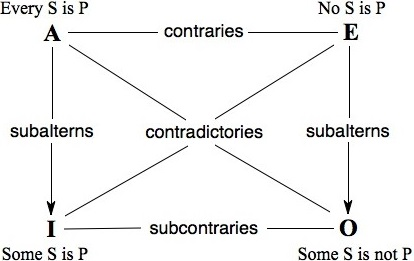
\includegraphics[width=0.7\textwidth]{SquareOfOpposition.jpg}
\end{figure}

In this book, we aren't interested in the logical relations of subalternation, contrariety, or subcontrariety, just contradiction. %So the Square of Opposition isn't a lot of use to us. %, Still, it's nice to know that $A$ and $O$ are contradictory, and $E$ and $I$ are contradictory.
This means that the Aristotelian Square of Opposition, the jewel of logic carefully passed down on scrolls for 2,000 years, reduces to a straight-forward observation about contradiction. %of the kind we saw at the beginning of this chapter.

Aristotle's  $A$-type statement `All Stamps are Paper' can be symbolised as $\qab{x}{Sx \eif Px}$, which is the same as $\enot\qeb{x}{Sx \eand \enot Px}$, which symbolises the negation of the $O$-type statement `Some Stamps aren't Paper'. That is, the $A$ and $O$-type statements are negations of each other, and so are  contradictory. 
%Similarly, the $E$-type statement `All Stamps aren't Paper', symbolised as $\qab{x}{Sx \eif \enot Px}$, is the same as $\enot\qeb{x}{Sx \eand Px}$, the negation of the $I$-type statement `Some Stamps are Paper'. The $E$ and $I$-type statements are contradictory.
Similarly, the $E$ and $I$-type statements are contradictory.


%This direct compositional conversion based on combining the features of each element of the statement provides a straight-forward way to symbolise all Aristotelian Syllogistic statements in \pl. This does \textbf{NOT} mean 

Note that Aristotelian Syllogisms are \textbf{NOT} a simple version of \pl; have a different notion validity, and so are a different logic system. But for our current purposes, they do provide a ring-fenced set of highly structured statements for exploration and practice. The Universal Affirmative, Universal Negative, Particular Affirmative, and Particular Negative statement types are still the key building blocks of \pl, 2,300 years later.





%Finite List of valid syllogisms
%Aristotle had a slightly different notion of validity than we use. This is not surprising, as he was the first person (that we know of) to formalise reasoning in this symbolic style. 

\logic{Over the next 2,000 years, the number of valid syllogisms varied between 15 and 24, as logicians subtly changed their ideas about validity, primarily by changing their minds about whether every Frog being Green meant that there were Green Frogs. This is the infamous \textit{Existential Import}. Actually, they didn't talk about Frogs, but properties of God; this had major theological significance, and sometimes logic changed with the election of a new Pope.}



\pagebreak
\practiceproblems
Refer to this symbolisation key for the next two problem sets: 

\begin{ekey}
\item[\atom A x] $x$ is airborne. 
\item[\atom I x] $x$ is infectious.
\item[\atom H x] $x$ is infectious to humans.
\item[\atom V x] $x$ is a virus.
\end{ekey}


\noindent\problempart
\label{pr.pl.symbol4}
Symbolise the following statements in \pl:
\begin{earg}
\item All viruses are infectious.
\item Not all viruses are infectious.
\item All viruses are not infectious. 
\item Some viruses are infectious.
\item No virus is infectious.
\item Some viruses are not infectious. 
\item Some viruses are infectious, but not to humans.
\item All viruses are infectious, but none is infectious to humans unless it's airborne.
\item If all viruses are airborne, then some are infectious to humans.
\item If no virus is airborne, then none is infectious to humans.
\item Not all viruses that are infectious to humans are airborne.
\item Some viruses that aren't infectious to humans are airborne.
\end{earg}

\noindent\problempart Using the logical equivalence between negated quantifiers ($\enot \qe$ vs. $\qa \enot$; and $\enot \qa$ vs. $\qe \enot$), as well as equivalences known from \tfl, link the statements from the first column to those in the second column that are logically equivalent: 

\[
  \begin{array}{lp{=2cm}l}
    \enot \qab{x}{\atom F x}&&\qeb{x}{\enot\enot \atom F x}\\
    \qab{x}{ \enot \atom F x}&&\qeb{x}{\neg \atom F x}\\
    \enot \qab{x}{ \enot \atom F x }&& \enot \qeb{x}{\enot \atom F x}\\
    \enot \enot \qab{x}{\atom F x} && \enot \qeb{x}{\atom F x}\\
    \qeb{x}{\enot (\atom P x \eand \atom Q x)} &&
	 \enot \qeb{x}{ \atom P x} \lor \enot \qeb{x}{\atom Q x} \\
    \enot \qab{x}{\atom P x \eand \atom Q x} &&
     \enot \qab{x}{\atom P x \eand \enot \atom Q x}\\
    \enot \enot \qeb{x}{\atom P x \eif \atom Q x} &&
     \enot \qab{x}{\atom P x \eand \atom Q x}\\
	\qeb{x}{\atom P x} \eif \qab{x}{\enot \atom Q x} &&
	 \qeb{x}{\enot \atom P x \eor \enot \atom Q x}\\
  \end{array}
\]


\pagebreak

\noindent\problempart
Provide two symbolisation keys for the following argument, and discuss how the treatment of ambiguous predicates affect the validity of the argument:

\begin{quote}
Willi is a fluffy cat, but a lousy mouser. Therefore, Willi is a lousy cat. 
\end{quote}


\noindent\problempart
\label{pr.pl.symbol6}
Using the following symbolisation key:

	\begin{ekey}
	\item[\atom K x ] x knows the combination to the safe
	\item[\atom P x ] x is a person
	\item[\atom S x ] x is a spy
	\item[\atom V x ] x is a vegetarian
	\end{ekey}
	\vspace{-54pt}\hspace{200pt}$h$:$\ \ \ $Hofthor
	
	\noindent\hspace{203pt}$i$:$\ \ \ $Ingmar
	\vspace{24pt}
%	\pagebreak
	
%	\begin{ekey}
%	\item[h] Hofthor
%	\item[i] Ingmar
%	\end{ekey}

\noindent Symbolise the following statements in \pl:
\begin{earg}
\item Neither Hofthor nor Ingmar is a vegetarian.
\item No spy knows the combination to the safe.
\item No one knows the combination to the safe unless Ingmar does.
\item Hofthor is a spy, but no vegetarian is a spy.
\end{earg}


\noindent\solutions
\problempart\label{pr.plalligators}
Using this symbolisation key:
\begin{ekey}
%\item[\text{domain}] all animals
\item[\atom A x ] x is an alligator.
\item[\atom M x ] x is a monkey.
\item[\atom R x ] x is a reptile.
\item[\atom Z x ] x lives at the zoo.
\item[a] Amos
\item[b] Bouncer
\item[c] Cleo
\end{ekey}
Symbolise each of the following statements in \pl:
\begin{earg}
\item Amos, Bouncer, and Cleo all live at the zoo. 
\item Bouncer is a reptile, but not an alligator. 
%\item If Cleo loves Bouncer, then Bouncer is a monkey. 
%\item If both Bouncer and Cleo are alligators, then Amos loves them both.
\item Some reptile lives at the zoo. 
\item Every alligator is a reptile. 
\item Anything that lives at the zoo is either a monkey or an alligator. 
\item There are reptiles which are not alligators.
%\item Cleo loves a reptile.
%\item Bouncer loves all the monkeys that live at the zoo.
%\item All the monkeys that Amos loves love him back.
\item If any animal is an reptile, then Amos is.
\item If any animal is an alligator, then it is a reptile.
%\item Every monkey that Cleo loves is also loved by Amos.
%\item There is a monkey that loves Bouncer, but sadly Bouncer does not reciprocate this love.
\end{earg}


\pagebreak
\noindent\problempart
\label{pr.arguments}
For each argument, write a symbolisation key and symbolise the argument in \pl.

\begin{earg}
\item Phoenix is a logician. All logicians wear funny hats. So Phoenix wears a funny hat.
\item Nothing on my desk escapes my attention. There is a computer on my desk. Thus there is a computer that does not escape my attention.
\item All my dreams are black and white. Old TV shows are in black and white. Therefore, some of my dreams are old TV shows.
\item Neither Holmes nor Watson has been to Australia. A person could see a kangaroo only if they had been to Australia or to a zoo. Although Watson has not seen a kangaroo, Holmes has. Therefore, Holmes has been to a zoo.
\item No one expects the Spanish Inquisition. No one knows the troubles I've seen. Therefore, anyone who expects the Spanish Inquisition knows the troubles I've seen.
%\item All babies are illogical. Nobody who is illogical can manage a crocodile. Berthold is a baby. Therefore, Berthold is unable to manage a crocodile.
\end{earg}


%\pg{I don't like this exercise, because it suggests that Aristotelean logic just is baby classical logic. }
\noindent\problempart
\label{pr.BarbaraEtc}
These are some of the syllogistic figures identified by Aristotle and his successors, along with their medieval names. 

Symbolise each argument in \pl.
\begin{earg}
\item[Barbara]: All $B$s are $C$s. All $A$s are $B$s.
	\therefore\  All $A$s are $C$s.
\item[Baroco]: All $C$s are $B$s. Some $A$ is not $B$.
	\therefore\  Some $A$ is not $C$.
\item[Baralipton]: All $B$s are $C$s. All $A$s are $B$s.
	\therefore\  Some $C$ is $A$.
\item[Bocardo]: Some $B$ is not $C$. All $A$s are $B$s.
	\therefore\  Some $A$ is not $C$.
\item[Celantes]: No $B$s are $C$s. All $A$s are $B$s.
	\therefore\  No $C$s are $A$s.
\item[Celarent]: No $B$s are $C$s. All $A$s are $B$s.
	\therefore\  No $A$s are $C$s.
\item[Cemestres]: No $C$s are $B$s. No $A$s are $B$s.
	\therefore\  No $A$s are $C$s.
\item[Cesare]: No $C$s are $B$s. All $A$s are $B$s.
	\therefore\  No $A$s are $C$s.
\item[Dabitis]: All $B$s are $C$s. Some $A$ is $B$.
	\therefore\  Some $C$ is $A$.
\item[Darii]: All $B$s are $C$s. Some $A$ is $B$.
	\therefore\  Some $A$ is $C$.
\item[Datisi]: All $B$s are $C$s. Some $A$ is $B$.
	\therefore\  Some $A$ is $C$.
\item[Disamis]: Some $B$ is $C$. All $A$s are $B$s.
	\therefore\  Some $A$ is $C$.
\item[Ferison]: No $B$s are $C$s. Some $A$ is $B$.
	\therefore\  Some $A$ is not $C$.
\item[Ferio:] No $B$s are $C$s. Some $A$ is $B$.
	\therefore\  Some $A$ is not $C$.
\item[Festino]: No $C$s are $B$s. Some $A$ is $B$.
	\therefore\  Some $A$ is not $C$.
\item[Frisesomorum]: Some $B$ is $C$. No $A$s are $B$s.
	\therefore\  Some $C$ is not $A$.
\end{earg}

\noindent\problempart Bonus question. One or two of the syllogisms listed above aren't valid in \pl. See if you can figure out which ones, before we introduce the formal methods for testing validity in \pl.

%\part{Complex Symbolisation}\label{part:cmpx}


\chapter{Multiple generality}\label{ch:MultipleGenerality}

So far, we have only considered statements that require one-place predicates and one quantifier. The full power of \pl\ really becomes apparent when we start to use many-place predicates and multiple quantifiers. %For this insight, we largely have Gottlob Frege (1879) to thank, but also C.S.~Peirce.


\section{Many-place Predicates}

\begin{center}
  \href{https://youtu.be/agbTz5OrrtM}
  {\XeTeXLinkBox{\qrcode[height=25mm]{https://youtu.be/agbTz5OrrtM}}}
\end{center}

All of the predicates that we have considered so far concern properties that things might have. %Those predicates have one gap in them, and to make a statement, we simply need to slot in one term.
They are \define{one-place} predicates.
Other predicates concern the \emph{relation} between things, such as: 
\begin{earg}
\item[\ex{rela}] Patrick and Sylvie are siblings.
\item[\ex{relb}] Auckland is to the north of Dunedin.
\item[\ex{relc}] Hamilton is in between Auckland and Tauranga.
\end{earg}

\noindent Statement \ref{rela} is about two things, Patrick and Sylvie, and relates them by saying that they are siblings.
Statement \ref{relb} also relates two things, Auckland and Dunedin, by saying that one is to the north of the other.
Statement \ref{relc}, however, relates three things, Hamilton, Auckland and Tauranga with a relation of \emph{in-betweenness}.   
We call the relations in statements \ref{rela} and \ref{relb} \define{two-place} predicates, and the relation in statement \ref{relc} a \define{three-place} predicate.
% They need to be filled in with two terms in order to make a statement.
% Conversely, if we start with an English statement containing many singular terms, we can remove two singular terms, to obtain different two-place predicates. Consider the statement `Vinnie borrowed the family car from Nunzio'. By deleting two singular terms, we can obtain any of three different two-place predicates
% 	\begin{quote}
% 		Vinnie borrowed \blank\ from \blank\\
% 		\blank\ borrowed the family car from \blank\\
% 		\blank\ borrowed \blank\ from Nunzio
% 	\end{quote}
% and by removing all three singular terms, we  obtain a \define{three-place} predicate:
% 	\begin{quote}
% 		\blank\ borrowed \blank\ from \blank
% 	\end{quote}
In principle, there is no upper limit on the number of places that our predicates may have. In practice, more than three is rare.

% Now there is a little foible with the above. We have used the same symbol, `\blank', to indicate a gap formed by deleting a term from a statement. However,% (as Frege emphasized),
%  these are \emph{different} gaps. To obtain a statement, we can fill them in with the same term, but we can equally fill them in with different terms, and in various different orders. The following are all perfectly good statements, and they all mean very different things:
% 	\begin{quote}
% 		Karl loves Karl\\
% 		Karl loves Imre\\
% 		Imre loves Karl\\
% 		Imre loves Imre
% 	\end{quote}
% The point is that we need to keep track of the gaps in predicates, so that we can keep track of how we are filling them in.


To keep track of the number of places in relations, as well as their order, we use variables. 
This is best explained by an example.
Suppose we want to symbolise the following statements:
\begin{earg}
  % \item[\ex{terms3}] Imre is at least as tall Karl.
  % \item[\ex{terms4}] Imre is shorter than Karl.
\item[\ex{terms3}] Karl loves Jesse.
\item[\ex{terms4}] Jesse is loved by Karl. 
\item[\ex{terms5}] Jesse loves themselves. 
\item[\ex{terms6}] Karl loves Jesse, but Jesse doesn't love Karl. 
\end{earg}
We will start with the following symbolisation key:
\begin{ekey}
\item[j] Jesse
\item[k] Karl
\item[\atom L xy ] x loves y
\end{ekey}
% Statement \ref{terms3} can now be symbolised by `$\atom T md$'. Note the order of the names! 
% Statement \ref{terms4} might seem as if it requires a new predicate. But there is obviously a connection connection between `shorter' and `taller.' We can paraphrase statement \ref{terms4} using predicates already in our key: `It is not the case that Imre is as tall or taller than Karl'. We can now symbolise it as `$\enot Tmd$'.

\noindent The symbolisation key has two names, $j$ and $k$, and a two-place predicate $\atom L  xy $.
The use of the variables $x$ and $y$ show that $L$ is a two-place predicate.
Furthermore, the order in which they appear in $\atom L  xy $ and in the English key shows that it is $x$ that loves $y$, and not the other way around.
Statements \ref{terms3} and \ref{terms4} both express that Karl loves Jesse, but in different voices: `Karl loves Jesse' is in the active voice, `Jesse is loved by Karl' in the passive voice.
This difference in voices is lost in \pl; we symbolise statements \ref{terms3} and \ref{terms4} in the same way:

\[
  \begin{array}{l}
    \atom L {k,j} \\
  \end{array}
\]

% Statement \ref{terms3} will now be symbolised by `$\atom L ki$'. 
% \noindent Statement \ref{terms4} can be paraphrased as `Imre loves Imre'. It can now be symbolised by `$\atom L ii$'.
\noindent Statement \ref{terms5} expresses that Jesse loves Jesse, which illustrates that the same name may occur more than once in a relation:
$$\atom L jj$$

\noindent Statement \ref{terms6} is a conjunction.
The first conjunct expresses that Karl loves Jesse, which we symbolise as
$$\atom L {k,j}$$

\noindent The second conjunct says that Jesses doesn't love Karl back:
%It denies that the lovig relation holds between Jesse and Karl (in that order): 
$$\enot \atom L {j,k}$$ 

\noindent This again illustrates the importance of the order of the places in predicates: 
Karl loves Jesse, but Jesse doesn't love Karl.
Another way of saying this is that the loving relation holds from Karl to Jesse, but not from Jesse to Karl. 
Putting things together, we symbolise statement \ref{terms6} like this: 

$$\atom L kj \eand \enot \atom L jk$$


When we are dealing with predicates with more than one place, we need to pay careful attention to the order of the places.


\section{Quantifier Order}

\begin{center}
  \href{https://youtu.be/Bny-1Fr4Tu0}
  {\XeTeXLinkBox{\qrcode[height=25mm]{https://youtu.be/Bny-1Fr4Tu0}}}
\end{center}

Consider the ambiguous statement `everyone loves someone'.
Why is it ambiguous? 
Because it could mean either of the following:
\begin{earg}
\item[\ex{lovecycle}] Everyone loves a person, though not necessarily the same person. 
\item[\ex{loveconverge}] There is some particular person whom everyone loves. 
\end{earg}

\noindent The language of \pl\ may not be the most beautiful language you've encountered, but it is very good at avoiding ambiguity.
It avoids ambiguity not only by using the order of variables in predicates, but also the order of quantifiers in formulas.
The difference between \ref{lovecycle} and \ref{loveconverge} is that the first expresses a $\qa \qe$ pattern of quantification whereas the second expresses a $\qe \qa$ pattern.
More precisely, take this symbolisation key:

\begin{ekey}
\item[\atom P x] x is a person
\item[\atom L xy ] x loves y
\end{ekey}

\noindent We can then symbolise statements \ref{lovecycle} and \ref{loveconverge} like this:

\[
  \begin{array}{l}
\qa{x}{\qeb{y}{(\atom P x \eand \atom Py) \eif \atom L  xy }}\\
\qe{x}{\qab{y}{(\atom P x \eand \atom Py) \eif \atom L yx}}
  \end{array}
  \]


The point of the example is to illustrate that the order of the quantifiers matters a great deal. Indeed, to switch them around is called a \emph{quantifier shift fallacy}. Here is an example, which comes up in various forms throughout the philosophical literature:
	\begin{earg}
		\item[] For every person, there is some truth they cannot know. \hfill ($\qa \qe$)
		\item[\therefore] There is some truth that no person can know. \hfill ($\qe \qa$)
	\end{earg}
        This argument form is invalid.
        It's just as bad as:
	\begin{earg}
		\item[] Everyday someone is struck by lightning. \hfill ($\qa \qe$)
		\item[\therefore] Some poor person is struck by lightning everyday. \hfill ($\qe \qa$)
	\end{earg}

   % The order of quantifiers is also important in definitions in mathematics.  For instance, there is a big difference between pointwise and uniform continuity of functions:
% \begin{itemize}
% \item A function $f$ is \emph{pointwise continuous} if
% \[
% \forall \epsilon\forall x\forall y\exists \delta(\left|x - y\right| < \delta \to \left|f(x) - f(y)\right| < \epsilon)
% \]
% \item A function $f$ is \emph{uniformly continuous} if
% \[
% \forall \epsilon\exists \delta\forall x\forall y(\left|x - y\right| < \delta \to \left|f(x) - f(y)\right| < \epsilon)
% \]
% \end{itemize}

\noindent This is why we ask you to take great care with the order of quantification.




\section{Stepping-stones to Symbolisation}

\begin{center}
  \href{https://youtu.be/YzbYDM11Ut0}
  {\XeTeXLinkBox{\qrcode[height=25mm]{https://youtu.be/YzbYDM11Ut0}}}
\end{center}

Once we have the possibility of multiple quantifiers and many-place predicates, symbolisation in \pl\ can become quite tricky. However, there are several stepping stones you can make use of. These steps are best illustrated by example. Consider this symbolisation key:
\begin{ekey}
\item[g] Geraldo
\item[\atom D x ] x is a dog
\item[\atom F xy ] x is a friend of y
\item[\atom O xy ] x owns y
\end{ekey}
Now let's try to symbolise these statements:
\begin{earg}
\item[\ex{dog2}] Geraldo is a dog owner.
\item[\ex{dog3}] There are dog owners.
\item[\ex{dog4}] All of Geraldo's friends are dog owners.
\item[\ex{dog5}] Every dog owner is a friend of a dog owner.
\item[\ex{dog6}] Every dog owner's friend owns a dog of a friend.
\end{earg}

\noindent Paraphrasing can help with identifying the quantifiers that are appropriate for symbolising a statement.
Statement \ref{dog2} can first be paraphrased as saying that `Geraldo owns a dog'.
This is what it means to be a dog owner.
Next, is this a universal or an existential statement?
The statement doesn't say that Geraldo owns every dog, but that Geraldo owns at least one dog, so we can paraphrase it as `There is a dog that Geraldo owns'.
This is easier to symbolise: 

$$\qeb{x}{\atom D x  \eand \atom O gx}$$

\noindent Statement \ref{dog3} says that at least one person is the owner of a dog, so it refers to two objects (the person and the dog) that don't have names, so will have two quantifiers, and their associated variables.
It may help to take them one at the time.
Let's first paraphrase \ref{dog3} as, `There is some x such that x owns a dog'.
This takes care of the first quantifier, so we can write, as an intermediary step, `$\qeb{x}{x\text{ owns a dog}}$'.
Now the fragment we have left as `$x$ owns a dog' is much like statement~\ref{dog2}, except that it is not specifically about Geraldo.
So we can symbolise statement~\ref{dog3} by:

$$\qe{x}{\qeb{y}{\atom D y  \eand \atom O  xy }}$$

We should pause to clarify something here. In working out how to symbolise the last statement, we wrote down `$\qeb{x}{x\text{ owns a dog}}$'.
To be very clear: this is \emph{neither} an \pl\ statement \emph{nor} an English statement, because it uses bits of \pl\ (`$\qe$', `$x$') and bits of English (`owns a dog').
It is really is \emph{just a stepping-stone} on the way to symbolising the entire English statement with a \pl\ statement.


Statement \ref{dog4} talks about all of Geraldo's friends, so it is a universal statement.
That's why we first paraphrase it as, `Every friend of Geraldo also owns a dog'.
Using our stepping-stone tactic, we might write

$$\qab{x}{\atom F xg \eif x \text{ is a dog owner}}$$

\noindent This leaves us to deal with the fragment `$x$ owns a dog', which we've already encountered in statement \ref{dog2}.
Because the variable $x$ is already used to talk about Geraldo's friends, we need to introduce a new variable, $y$: 

$$\qab{x}{\atom F xg \eif \qeb{y}{\atom D y  \eand \atom O xy }}$$

%\notation{You may have noticed that we used [square brackets] as well as (parentheses) in the previous formula. In this course, all types of bracket mean the same thing; it's just easier to see which brackets are which if we vary what they look like.}


Speeding up the intermediate steps, statement \ref{dog5} can be paraphrased as `For any $x$ that owns a dog, there is someone who owns a dog and whom $x$ is a friend of'.
Using our stepping-stone tactic, this becomes 
$$\qab{x}{\mbox{$x$ owns a dog}\eif \qeb{y}{\mbox{$y$ owns a dog}\eand \atom F xy }}$$
Completing the symbolisation, we end up with
$$\qab{x}{\qeb{z}{\atom D z \eand \atom O xz}\eif \qeb{y}{\qeb{w}{\atom D w \eand \atom O yw}\eand \atom F xy }}$$

Statement \ref{dog6} is the trickiest yet. First we paraphrase it as `For any $x$ that is a friend of someone who owns a dog, $x$ owns a dog, and that dog is also owned by a friend of~$x$'. Using our stepping-stone tactic, this becomes:
\begin{multline*}
\qab{x}{ x\text{ is a friend of someone who owns a dog}\eif {}\\
x\text{ owns a dog which is also owned by a friend of }x}
\end{multline*}

Breaking this down a bit more:

\begin{multline*}
	\qab{x}{\qeb{y}{\atom F xy  \eand y\text{ owns a dog}}\eif {}\\
\qeb{z}{\atom D z \eand \atom O xz \eand z\text{ is owned by a friend of }x}}
\end{multline*}
And a bit more: 
\begin{multline*}
\qab{x}{\qeb{y}{\atom F xy  \eand \qeb{w}{\atom D w \eand \atom O yw}} \eif {} 
\qeb{z}{\atom D z \eand \atom O xz \eand \qeb{v}{\atom F vx \eand \atom O vz}}}
\end{multline*}
And we are done.
We told you, things get tricky quickly!

Hopefully, using these stepping-stones between English and \pl\ will help you simplifying the problem of symbolising complex statements into formulas by breaking down the tasks into simpler ones. 

\section{De-Symbolising}

\begin{center}
  \href{https://youtu.be/XY7_q3fj1SU}
  {\XeTeXLinkBox{\qrcode[height=25mm]{https://youtu.be/XY7_q3fj1SU}}}
\end{center}

So far we've looked at symbolising statements, which goes from a natural language (English) to a formal language (\pl). When you start working with formal languages like \pl, however, you will be working directly with the symbolisation, but will still have to communicate about it in natural language. You will then need to be able to read formulas, or as we like to put it, to \emph{de-symbolise}. Using a stepping-stone approach is very useful for that. Let's see some examples, working with this symbolisation key:

\begin{ekey}
\item[\atom I x] x is an instrument.
\item[\atom M x ] x is a musician.
\item[\atom P xy ] x plays y.
\end{ekey}

\noindent We will desymbolise these two formulas back to English:

\begin{earg}
\item[\ex{music1}] $\qab{x}{\atom M x \eif \qeb{y}{\atom I y \eand \atom P  xy }}$
\item[\ex{music2}] $\qeb{x}{\atom M x \eand \qab{y}{\atom I y \eif \atom P  xy }}$
\end{earg}

\noindent Start with formula \ref{music1}. One step in desymbolising a formula is to simply read every symbol out loud, as in:

\begin{quote}
For every $x$, if $x$ is a musician, then there is a $y$ such that $y$ is an instrument and $x$ plays $y$. 
\end{quote}

\noindent This is (nearly) a sentence of English, as you have transformed most parts of the formula into English, but it's only a stepping stone towards a naturally flowing English sentence.
%Instead of translating, reading out loud in this way is more like transliterating.
Our stepping-stone approach to desymbolising has as an end-goal to produce a nice sentence of English.

Let's try again, taking each part of the  formula in turn.
One useful way to divide up a complex formula is quantifier by quantifier. Formula \ref{music1} has two quantifiers. We will start by transforming the outermost quantifier:

\begin{quote}
  For every $x$, if $x$ is a musician, then $\qeb{y}{\atom I y \eand \atom P  xy }$
\end{quote}


\noindent Now that we know what we are talking about, namely everything that is a musician, we can express this part of the formula in English with:

\begin{quote}
  Every musician \dots $\qeb{y}{\atom I y \eand \atom P  xy }$
\end{quote}

\noindent Next we transform the existential quantifier:


\begin{quote}
  Every musician \dots there is a $y$ such that $y$ is an instrument and $P xy $.
\end{quote}

\noindent This tells us that every musician does something to an instrument.
What is it?

\begin{quote}
  Every musician \dots there is a $y$ such that $y$ is an instrument and $x$ plays $y$.
\end{quote}

\noindent Now we have all the information we need: for every musician there is an instrument that the musician plays, or written elegantly:

\begin{quote}
  Every musician plays an instrument.
\end{quote} 

\noindent And this is how we desymbolise formula \ref{music1} into English.
For formula \ref{music2}, we follow a similar procedure.
We transform the outermost quantifier first:

\begin{quote}
  There is a $x$ such that $x$ is a musician and $\qab{y}{\atom I y \eif \atom P  xy }$
\end{quote}

\noindent So we know that something is going on with a musician:

\begin{quote}
  Some musician \dots $\qab{y}{\atom I y \eif \atom P  xy }$
\end{quote}

\noindent Next we transform the universal quantifier:

\begin{quote}
  Some musician \dots for all $y$, if $y$ is an instrument, then $\atom P  xy $. 
\end{quote}

\noindent What does the musician do to every instruments?
They play it:

\begin{quote}
  Some musician \dots for all $y$, if $y$ is an instrument, then $x$ plays $y$. 
\end{quote}  

\noindent Now we have all the information needed to express it in English:

\begin{quote}
  Some musician plays all instruments. 
\end{quote} 



\section{Suppressed Quantifiers}

Logic can often help to clarify statements, especially where the quantifiers are left implicit or their order is ambiguous or unclear. The clarity of expression and thinking afforded by \pl\ can give you a significant advantage in argument, as can be seen in the following takedown by British political philosopher Mary Astell (1666--1731) of her contemporary, the theologian William Nicholls. In Discourse IV: The Duty of Wives to their Husbands of his \textit{The Duty of Inferiors towards their Superiors, in Five Practical Discourses} (London 1701), Nicholls argued that women are naturally inferior to men. In the preface to the 3rd edition of her treatise \emph{Some Reflections upon Marriage, Occasion'd by the Duke and Duchess of Mazarine's Case; which is also considered,} Astell responded as follows:
\begin{quotation}
'Tis true, thro' Want of Learning, and of that Superior Genius which Men as Men lay claim to, she [Astell] was ignorant of the \textit{Natural Inferiority} of our Sex, which our Masters lay down as a Self-Evident and Fundamental Truth. She saw nothing in the Reason of Things, to make this either a Principle or a Conclusion, but much to the contrary; it being Sedition at least, if not Treason to assert it in this Reign. 

For if by the Natural Superiority of their Sex, they mean that \textit{every} Man is by Nature superior to \textit{every} Woman, which is the obvious meaning, and that which must be stuck to if they would speak Sense, it wou'd be a Sin in \textit{any} Woman to have Dominion over \textit{any} Man, and the greatest Queen ought not to command but to obey her Footman, because no Municipal Laws can supersede or change the Law of Nature; so that if the Dominion of the Men be such, the \textit{Salique Law,}\footnote{The Salique law was the common law of France which prohibited the crown be passed on to female heirs.} as unjust as \textit{English Men} have ever thought it, ought to take place over all the Earth, and the most glorious Reigns in the \textit{English, Danish, Castilian}, and other Annals, were wicked Violations of the Law of Nature!

If they mean that \textit{some} Men are superior to \textit{some} Women this is no great Discovery; had they turn'd the Tables they might have seen that \textit{some} Women are Superior to \textit{some} Men. Or had they been pleased to remember their Oaths of Allegiance and Supremacy, they might have known that \textit{One} Woman is superior to \textit{All} the Men in these Nations, or else they have sworn to very little purpose.\footnote{In 1706, England was ruled by  Queen Anne.} And it must not be suppos'd, that their Reason and Religion wou'd suffer them to take Oaths, contrary to the Laws of Nature and Reason of things.\footnote{Mary Astell, \textit{Reflections upon Marriage}, 1706 Preface, iii--iv, and Mary Astell,
  \textit{Political Writings}, ed. Patricia Springborg, Cambridge   University Press, 1996, 9--10.}
\end{quotation}
We can symbolise the different interpretations Astell offers of Nicholls' claim that men are superior to women:
He either meant that every man is superior to every woman, i.e.,
$$\qab{x}{\atom M x  \eif \qab{y}{\atom W y \eif \atom S xy }}$$

or that some men are superior to some women,
$$\qeb{x}{\atom M x  \eand \qeb{y}{\atom W y \eand \atom S xy }}.$$

The latter is true, but then so is
$$\qeb{y}{\atom W y \eand \qeb{x}{\atom M x  \eand \atom S yx}}.$$

(some women are superior to some men), so that, Astell says,  would be ``no great discovery''.  In fact, since the Queen is superior to all her subjects, it's even true that some woman is superior to every man, i.e.,
$$
\qeb{y}{\atom W y \land \qab{x}{\atom M x  \eif \atom S yx}}.$$
But this is incompatible with the ``obvious meaning'' of Nicholls' claim, i.e., the first reading. So what Nicholls claims amounts to treason against the Queen!


\pagebreak
\practiceproblems
\problempart
\label{pr.love1}
Using the following symbolisation key:
\begin{ekey}
\item[i] me
\item[\atom P x ] x is a person.
\item[\atom W x ] x is a winner.
\item[\atom T x ] x is a time.
\item[\atom L xy ] x loves y.
\item[\atom H xyz] x loves y at z.
\end{ekey}

\noindent symbolise the following statements in \pl:
\begin{earg}
\item Everybody loves a winner. 
\item Nobody loves me. 
\item Everybody loves somebody sometime. 
\end{earg}


\problempart
\label{pr.love2}
Using the following symbolisation key:
\begin{ekey}
\item[i] me
\item[\atom P x ] x is a person.
\item[\atom W x ] x is a winner.
\item[\atom T x ] x is a time.
\item[\atom L xy ] x loves y.
\item[\atom H xyz] x loves y at z.
\end{ekey}

\noindent Desymbolise the following formulas of \pl\ into English: 
\begin{earg}
\item $\qeb{x}{\atom P x \eand \qab{y}{\atom W y \eif \atom L  xy }}$
\item $\enot \qab{x}{ \atom L xi}$
\item $\qeb{x}{\atom P x \eand \qab{y}{\atom P y \eif \qeb{z}{\atom T z \eand \atom H xyz}}}$ 
\end{earg}


\noindent\solutions
\problempart
Using this symbolisation key:
\begin{ekey}
\item[a] Amos
\item[b] Bouncer
\item[c] Cleo
\item[\atom A x ] x is an alligator
\item[\atom M x ] x is a monkey
\item[\atom R x ] x is a reptile
\item[\atom Z x ] x lives at the zoo
\item[\atom L xy ] x loves y
\end{ekey}
symbolise each of the following statements in \pl:
\begin{earg}
%\item Amos, Bouncer, and Cleo all live at the zoo. 
%\item Bouncer is a reptile, but not an alligator. 
\item If Cleo loves Bouncer, then Bouncer is a monkey. 
\item If both Bouncer and Cleo are alligators, then Amos loves them both.
%\item Some reptile lives at the zoo. 
%\item Every alligator is a reptile. 
%\item Any animal that lives at the zoo is either a monkey or an alligator. 
%\item There are reptiles which are not alligators.
\item Cleo loves a reptile.
\item Bouncer loves all the monkeys that live at the zoo.
\item All the monkeys that Amos loves love him back.
%\item If any animal is an reptile, then Amos is.
%\item If any animal is an alligator, then it is a reptile.
\item Every monkey that Cleo loves is also loved by Amos.
\item There is a monkey that loves Bouncer, but sadly Bouncer does not reciprocate this love.
\end{earg}


\noindent\problempart 
Using this symbolisation key:
\begin{ekey}
\item[r] Rave
\item[h] Shane
\item[d] Daisy
\item[\atom A x] x is an animal
\item[\atom D x ] x is a dog
\item[\atom S x ] x likes samurai movies
\item[\atom L xy ] x is larger than y
\end{ekey}

symbolise the following statements in \pl:

\begin{earg}
\item Rave is a dog who likes samurai movies.
\item Rave, Shane, and Daisy are all dogs.
\item Shane is larger than Rave, and Daisy is larger than Shane.
\item All dogs like samurai movies.
\item Only dogs like samurai movies.
\item There is a dog that is larger than Shane.
\item If there is a dog larger than Daisy, then there is a dog larger than Shane.
\item No animal that likes samurai movies is larger than Shane.
\item No dog is larger than Daisy.
\item Any animal that dislikes samurai movies is larger than Rave.
\item There is an animal that is between Rave and Shane in size.
\item There is no dog that is between Rave and Shane in size.
\item No dog is larger than itself.
\item Every dog is larger than some dog.
\item There is an animal that is smaller than every dog.
\item Any animal that is larger than any dog does not like samurai movies.
\end{earg}


\noindent\problempart
\label{pr.QLcandies}
Using this symbolisation key:
\begin{ekey}
\item[\atom C x ] x is a candy.
\item[\atom M x ] x has marzipan in it.
\item[\atom S x ] x has sugar in it.
\item[\atom T x ] Boris has tried x.
\item[\atom B xy ] x is better than y.
\end{ekey}
symbolise the following statements in \pl:
\begin{earg}
\item Boris has never tried any candy.
\item Marzipan is always made with sugar.
\item Some candy is sugar-free.
%\item The very best candy is chocolate.
\item No candy is better than itself.
\item Boris has never tried sugar-free candies.
%\item Boris has tried marzipan and chocolate, but never together.
%\item Boris has tried nothing that is better than sugar-free marzipan.
\item Any candy with sugar is better than any candy without it.
%\item Any candy with chocolate and marzipan is better than any candy that lacks both.
\end{earg}


\noindent\problempart
Using this symbolisation key:
\begin{ekey}
\item[e] Eli
\item[f] Francesca
\item[g] the guacamole
\item[\atom D x ] x is a dish.
\item[\atom F x ] x is food.
\item[\atom P x ] x is a person.
\item[\atom R x ] x has run out.
\item[\atom T x] x is on the table.
\item[\atom L xy ] x likes y.
\end{ekey}
symbolise the following English statements in \pl:
\begin{earg}
\item All the food is on the table.
\item If the guacamole has not run out, then it is on the table.
\item Everyone likes the guacamole.
\item If anyone likes the guacamole, then Eli does.
\item Francesca only likes the dishes that have run out.
\item Francesca likes no one, and no one likes Francesca.
\item Eli likes anyone who likes the guacamole.
\item Eli likes anyone who likes the people that he likes.
\item If there is a person on the table already, then all of the food must have run out.
\end{earg}


\noindent\solutions
\problempart
\label{pr.plballet}
Using this symbolisation key:
\begin{ekey}
\item[e] Elmer
\item[j] Jane
\item[p] Patrick
\item[\atom D x ] x dances ballet.
\item[\atom F x ] x is female.
\item[\atom M x ] x is male.
\item[\atom P x ] x is a person. 
\item[\atom C xy ] x is a child of y.
\item[\atom S xy ] x is a sibling of y.
\end{ekey}
symbolise the following statements in \pl:
\begin{earg}
\item All of Patrick's children are ballet dancers.
\item Jane is Patrick's daughter.
\item Patrick has a daughter.
\item Jane is an only child.
\item All of Patrick's sons dance ballet.
\item Patrick has no sons.
\item Jane is Elmer's niece.
\item Patrick is Elmer's brother.
\item Patrick's brothers have no children.
\item Jane is an aunt.
\item Everyone who dances ballet has a brother who also dances ballet.
\item Every woman who dances ballet is the child of someone who dances ballet.
\end{earg}


\chapter{Identity}
\label{ch:identity}

Consider this statement:
\begin{earg}
\item[\ex{else1}] Aristotle is more philosophical than anyone on YouTube. 
\end{earg}
% Let the domain be people; this will allow us to symbolise `everyone' as a universal quantifier.
Using the symbolisation key:

\begin{ekey}
\item[a] Aristotle
\item[\atom Y x] x is a person on Youtube
\item[\atom P xy ] x is more philosophical than y
\end{ekey}

\noindent we could attempt to symbolise statement \ref{else1} with: 

$$\qab{x}{Yx \eif \atom P ax }$$

\noindent This symbolisation isn't accurate, however.
Can you see why?
The problem is that Aristotle is also on YouTube, and if Aristotle is more philosophical than anyone on YouTube, then Aristotle is more philosophical than themself, which is absurd.
What statement \ref{else1} is meant to say is rather something like this: 
\begin{earg}
\item[\ex{else2}] Aristotle is more philosophical than \emph{anyone else} on YouTube. 
\end{earg}

\noindent but we do not have the resources in \pl\ to express \emph{anyone else}.
What we have in \pl\ are two quantifiers, the universal quantifier $\qa$ that talks about everything, and the existential quantifier $\qe$ that talks about at least one thing.
Neither quantifier allows us to talk about everything \emph{except} Aristotle.
You might be tempted by this symbolisation:


$$\qab{x}{Yx \eif \atom P ax} \eand \enot \atom P aa$$

\noindent This says that Aristotle is more philosophical than anyone on YouTube (including Aristotle) and that Aristotle isn't more philosophical than Aristotle.
But this formula is a contradiction, and that won't do.
The solution is to add identity to \pl.
Identity is the subject of this chapter. 

\section{Adding Identity}

\begin{center}
  \href{https://youtu.be/fwjIfGJFFps}
  {\XeTeXLinkBox{\qrcode[height=25mm]{https://youtu.be/fwjIfGJFFps}}}
\end{center}

An \define{identity} between terms expresses that we have two ways of talking about one thing.
For instance, identity holds between Diana Prince and Wonder Woman, because they are the same person.
In \pl, we treat identity as a special predicate and we add a special symbol for it, the symbol `$=$'. 
% The symbol `$=$' is a two-place predicate. Since it is to have a special meaning, we will write it a bit differently: we put it between two terms, rather than out front. 
We \emph{always} adopt the following symbolisation key for identity:
\begin{ekey}
\item[x=y] x is identical to y
\end{ekey}

\noindent To say that $x$ and $y$ are identical does not mean \emph{merely} that the objects they refer to are indistinguishable, or that all of the same things are true of them.
Rather, it means that $x$ and $y$ refer to \emph{the very same} object.

For the next examples, we will use this symbolisation key:

\begin{ekey}
\item[d] Diana Prince
\item[p] Peter Parker
\item[w] Wonder Woman
\item[x=y] x is identical to y
\end{ekey}

We use identity to symbolise statements like this: 
\begin{earg}
\item[\ex{else7}] Diana Prince is Wonder Woman.
\end{earg}

\noindent We can then symbolise statement \ref{else7} in this way:

$$d = w$$

\noindent Simple!
This means that the names `$d$' and `$w$' both refer to (name) the same thing.
One notational difference about identity is that we write $d = w$ instead of $= (d, w)$ like other predicates.
This makes it easier to read.

\compsci{This way of writing identity is what is an \emph{infix} notation, because the identity symbol is written in between its two arguments x and y.
  In contrast, we have been using a \emph{prefix} notation for our predicates.
  In terms of expressivity, the difference in notation doesn't make a difference.
For some coding purposes, however, prefix notation is taken to be easier to work with, especially with complex codes.}

Like other predicates, we can express that identity doesn't hold between two things with a negation.
For instance, we could symbolise that Peter Parker isn't Wonder Woman like this:

$$\enot (p = w)$$

\noindent but this is not very pretty.
We prefer to use the following notation:

$$p \neq w$$

\noindent which expresses that Peter Parker isn't (identical to) Wonder Woman. \\

With this new symbol added to \pl, we can now come back to our example about Aristotle.
We now use this symbolisation key:

\begin{ekey}
\item[a] Aristotle
\item[\atom Y x] x is a person on Youtube
\item[\atom P xy ] x is more philosophical than y
\item[x=y] x is identical to y
\end{ekey}

\noindent To express that Aristotle is more philosophical than \emph{anyone else} on YouTube, we use identity to exclude Aristotle:

$$ \qab{x}{(\atom Yx \eand x \neq a) \eif \atom P ax}$$

\noindent This formula says that Aristotle is more philosophical than anyone on Youtube, except themself.
We can also use identity to symbolise something more complex, like:

\begin{earg}
\item[\ex{most}] Aristotle is the most philosophical person on YouTube
\end{earg}

\noindent How might we express this in \pl? Here's one reasonable symbolisation:

% $$\qab{x}{\atom Y x \eif \qab{y}{(\atom Y y \eand y \neq x) \eif \atom P  xy  } \eif x = s}$$

%\[\begin{array}{c}(\atom Y a \land \qab{x}{(\atom Y x\land x\neq a) \eif \atom P ay})\\ \land\\ \qab{y}{\atom Y y \eif (\qab{z}{(\atom Y z \eand z \neq y) \eif \atom P yz } \eif y = a)}\end{array}\]



$$\atom Y a \land \qab{x}{\atom Y x \eif (\qab{z}{(\atom Y x \eand z \neq x) \eif \atom P xz } \eiff x = a)}$$ 

\noindent This says that Aristotle is on Youtube, that if anyone is more philosophical than anyone else on Youtube then that person is Aristotle (to avoid ties), and that he is more philosophical than anyone else on Youtube.

\noindent \textit{Hint} To read this formula: break down the $\eiff$ into an $\eif$ and a $\rightarrow$, and pay attention to the bracketing, and the quantifier scope for $z$.

Having identity allows us to express more nuanced concepts. But we are also going to have to be more careful, and to accustom ourselves to reading and creating longer formulas.



\section{Using Identity} 

We have already seen a couple of ways to use identity. It's time to go through some common applications a little more systematically.\\

We can state that two English names are identical, as we did when declaring Diana Prince to be Wonder Woman. We symbolised this in \pl\ by $d=w$.

We can also do this with name-like definite descriptions. With this key:

\begin{ekey}
\item[k] The cutest kitten in Auckland.
\item[b] Belinda.
\item[a] Auckland.
\item[c(\textit{x})] The cutest kitten in \textit{x}.
\end{ekey}
`Belinda is  the cutest kitten in Auckland' can be symbolised as $b = k$. Or if we allow functions in our language, we could symbolise this statement as $b = c(a)$. It would also be true that $k = c(a)$.\\

We can also state that a name satisfies a quantifier.  With this key:

\begin{ekey}
\item[j] Jeremy.
\item[L x] x is your lecturer.
\end{ekey}
`One of your lecturers is Jeremy' can be symbolised by $\qeb{x}{Lx \eand x = j}$. You could also symbolise this simply as $Lj$, although that might be more suited to symbolising `Jeremy is your lecturer', a statement with a similar meaning but that we would use in different contexts. The opportunities for subtlety continue to grow!\\


We can also claim that names are non-identical, such as when we symbolised that Peter Parker was not Wonder Woman, by $p\neq w$. There are a number of common words whose meaning is a kind of non-identity. 

\paragraph{Other} 
To be `other' is to not be the same as. With this key:
\begin{ekey}
\item[i] Me.
\item[u] You.
\item[Px] \textit{x} is a person.
\item[Txy] \textit{x} is thinking of \textit{y}.
\end{ekey}

`I was thinking of someone other than you' can be symbolised by the formula $\qeb{x}{Px \eand Tix \eand x \neq u}$. We might want to add $(u \neq i)$ if we think that grammatical truth is important to the argument.


\pagebreak

\paragraph{Another / Else} 
To be `another' is something like being `other', but usually in addition to. `I was thinking of another person, not just of you' can be symbolised using the above key by the formula $\qeb{x}{Px \eand Tix \eand x \neq u} \eand Tiu$. We could also symbolise `I was not just thinking of you' similarly, although we don't know I'm thinking of another \textit{person}: $\qeb{x}{Tix \eand x \neq u} \eand Tiu$. And `I wasn't thinking of you at all' could be symbolised as $\enot Tiu$, but if we interpret this ambiguous statement as `I was thinking of someone else' it could be symbolised as $\qeb{x}{Px \eand Tix \eand x \neq u} \eand \enot Tiu$. 



\paragraph{No one else / No one but}
The phrase `no one else' is a negation of `someone else'. Suppose we stated `I was thinking of you and no one else', or `I was thinking of no one but you', or `All I thought of was you'. Then using the above key, we can symbolise these sweet whispers as $Tiu \eand \qab{x}{Tix \eif x = u}$ or more compactly $\qab{x}{Tix \eiff x = u}$. Isn't logic romantic!


\paragraph{Also}
`Also' is something like `and', but the two conjuncts must refer to distinct (non-identical) objects. With this key:
\begin{ekey}
\item[i] Me.
\item[u] You.
\item[Fxy] \textit{x} is a friend of  \textit{y}.
\item[Hxy] \textit{x} is hanging with \textit{y}.
\end{ekey}
We can symbolise `I hang out with all my friends, and also with you' as $\qab{x}{Fix \eif (Hix \eand x \neq u)} \eand Hiu$, which is pretty brutal. Contrast that with  `I hang out with all my friends, including you' which we would symbolise as $\qab{x}{Fix \eif Hix} \eand Fiu$.


\paragraph{Except / Unless}
`Except' works roughly like `unless', except that it can be used for excluding individuals. We can express most `except' statements using an `unless', replacing individuals in the exception with a statement. For example, `I hang out with all my friends, except you' means roughly the same as `I hang out with all my friends, unless they are you', or `I hang out with all my friends, if they are not you'.

We can symbolise any of these statements using the above key as $\qab{x}{(Fix\eand x \neq u) \eif Hix} \eand Fiu$. Compare this with the similar `also' sentence above. Here you are a friend, and we leave it open whether I hang out with you or not. If you think that the English sentence logically excludes that I hang out with you, we can change the formula from an `\eif' to a `\eiff': $\qab{x}{(Fix\eand x \neq u) \eiff Hix} \eand Fiu$.




\paragraph{Only}

As promised in Chapter \ref{ch:TFLComplications}, we are finally returning to discuss `only' in more detail. It's worth have another read of \S\ref{s.only} first. With this key:
\begin{ekey}
\item[j] Janice.
\item[Hx] \textit{x} can talk.
\end{ekey}

We can symbolise `Only humans talk' as $\qab{x}{\enot Hx \eif \enot Tx}$, or $\qab{x}{Tx \eif Hx}$. But it doesn't mean that all humans talk $\qab{x}{Hx \eif Tx}$, and so it can't be symbolised as $\qab{x}{Hx \eiff Tx}$. This is just like what we said when symbolising `only' in \tfl. But with identity, we can also consider individuals. And our rule of thumb of negating both the antecedent and consequent of our conditional still applies when we are making statements about individuals. The statement `Only Janice can talk' would be symbolised as $\qab{x}{x\neq j \eif \enot Tx}$; we do not include $Tj$, as it does not automatically also mean that in all contexts. 

\paragraph{The One and Only / The Only}
The expression `The one and only' is the name-level analogue to the propositional `if and only if'. It is often shortened to `the only'. This expression does include both halves of the logical content. The expression `Janice is the (one and) only person who can talk' is roughly `Janice is one person who can talk AND only Janice can talk', which can be would be symbolised as $Tj \eand \qab{x}{x\neq j \eif \enot Tx}$, or as the equivalent but more compact $\qab{x}{Tx \eiff x = j}$.


\paragraph{The}
This now gives us another approach to understanding and symbolising  definite descriptions. To say `the $A$' is to say that there is at least one thing that is $A$, and that only that thing is $A$. With this key:
\begin{ekey}
\item[a] The accountant.
\item[Ax] \textit{x} is an accountant.
\item[Sx] \textit{x} smirked.
\end{ekey}

We can symbolise `The accountant smirked' as either: $Sa$ by treating `the accountant' as standing for a name, or as $\qeb{x}{Ax \eand \qab{y}{Ay \eif x=y} \eand Sx}$. This latter approach would naturally lead us to consider statements where a definite description does not refer to exactly one object as being false. Considerations from our previous discussion on definite descriptions then help us decide whether we think this is an adequate symbolisation or not.




\pagebreak
\section{Counting on Identity}\label{s.counting}

\paragraph{At least\ldots}

\begin{center}
  \href{https://youtu.be/BvwJ69VBXZg}
  {\XeTeXLinkBox{\qrcode[height=25mm]{https://youtu.be/BvwJ69VBXZg}}}
\end{center}

We can also use identity to say how many things there are of a particular kind. For example, consider these statements:
\begin{earg}
\item[\ex{atleast1}] There is at least one apple
\item[\ex{atleast2}] There are at least two apples
\item[\ex{atleast3}] There are at least three apples
\end{earg}
We will use the symbolisation key:
	\begin{ekey}
		\item[\atom A x ] x is an apple
	\end{ekey}
Statement \ref{atleast1} does not require identity. It can be adequately symbolised by `$\qeb{x}{\atom A x }$': There is an apple; perhaps many, but at least one.

It might be tempting to also symbolise statement \ref{atleast2} without identity. Yet consider the statement `$\qe{x}{\qeb{y}{\atom A x  \eand \atom A y}}$'. Roughly, this says that there is something $x$ that is an apple and something $y$ that is an apple. But since nothing prevents these from being the same apple, this would be true even if there were only one apple. In order to make sure that we are dealing with \emph{different} apples, we need an identity predicate. Statement \ref{atleast2} needs to say that the two apples that exist are not identical, and so we symbolise it by:
\[
	\qe{x}{\qeb{y}{(\atom A x  \eand \atom A y) \eand x \neq y}}.
\]
Statement \ref{atleast3} requires talking about three different apples. Now we need three existential quantifiers, and we need to make sure that each will pick out something different: 
\[
	\qe{x}{\qe{y}{\qeb{z}{(\atom A x  \eand \atom A y \eand \atom A z) \eand (x\neq y \eand y \neq z \eand x\neq z)}}}.
\]
Note that it is \emph{not} enough to use `$x\neq y \land y\neq z$' to symbolise `$x$, $y$, and $z$ are all different.' For that would be true if $x$ and $y$ were different but $x = z$. Nor can we use the mathematical short-hand `$x\neq y \neq z$' As logicians, we aspire to avoid the casual notational abuse and general sloppiness of mathematicians.

\pagebreak


\paragraph{At most\ldots}
Now consider these statements:
\begin{earg}
	\item[\ex{atmost1}] There is at most one apple
	\item[\ex{atmost2}] There are at most two apples
\end{earg}
Statement \ref{atmost1} can be paraphrased as `It is not the case that there are at least \emph{two} apples'. This is just the negation of statement \ref{atleast2}: 
$$\enot \qe{x}{\qeb{y}{(\atom A x  \eand \atom A y ) \eand x\neq y}}$$
But statement \ref{atmost1} can also be approached in another way. It means that if you pick out an object and it's an apple, and then you pick out an object and it's also an apple, you must have picked out the same object both times. With this in mind, it can be symbolised by
$$\qa{x}{\qab{y}{(\atom A x  \eand \atom A y ) \eif x=y}}$$
The two statements will turn out to be logically equivalent.\\

In a similar way, statement \ref{atmost2} can be approached in two equivalent ways. It can be paraphrased as, `It is not the case that there are \emph{three} or more distinct apples', so we can write:
$$\enot \qe{x}{\qe{y}{\qeb{z}{\atom A x  \eand \atom A y  \eand \atom A z  \eand x\neq y \eand y \neq z \eand x\neq z}}}$$
Alternatively we can read it as saying that if you pick out an apple, and an apple, and an apple, then you will have picked out (at least) one of these objects more than once. Thus:
$$\qa{x}{\qa{y}{\qab{z}{(\atom A x  \eand \atom A y  \eand \atom A z ) \eif (x=y \eor x=z \eor y=z)}}}$$
Another way of saying that is `if you are showing me three apples, then you must have shown me at least one apple twice'.\\

This method of counting can get tiresome if we are dealing with complex predicates. For example, consider the statement `at least 2 cats chased a mouse or two into someone's room'. We might symbolise this as:

\begin{multline*}
	\qe{x}{}\qe{y}{}\qe{z}{}\qe{t}{}\qeb{u}{
	  (Cat(x) \eand Cat(y)   \eand Person(z) \eand Room (t) \eand Owns(zt) \\
  \eand Mouse(u) \eand Chased(xut) \eand Chased(yut) 
	  \eand (x\neq y ) \\
	  \eand \enot \qe{v}{}\qeb{w}{Mouse(v) \eand Mouse(w) \eand Chased(xvt) \eand Chased(yvt) \\
	  \eand Chased(xwt) \eand Chased(ywt) \eand (u\neq v \eand u\neq w \eand v \neq w)}
	}.
\end{multline*}


\pagebreak


\paragraph{Exactly\ldots}
We can now consider precise statements, like:
\begin{earg}
\item[\ex{exactly1}] There is exactly one apple.
\item[\ex{exactly2}] There are exactly two apples.
\item[\ex{exactly3}] There are exactly three apples.
\end{earg}
Statement \ref{exactly1} can be paraphrased as, `There is \emph{at least} one apple and there is \emph{at most} one apple'. This is just the conjunction of statement \ref{atleast1} and statement \ref{atmost1}. So we can write:
$$\qeb{x}{\atom A x } \eand \qa{x}{\qab{y}{(\atom A x  \eand \atom A y ) \eif x=y}}$$
But it is perhaps more straightforward to paraphrase statement \ref{exactly1} as, `There is a thing $x$ which is an apple, and everything which is an apple is just $x$ itself'. Thought of in this way, we write: 
\[
	\qeb{x}{\atom A x  \eand \qab{y}{\atom A y  \eif x= y}}
\]
Similarly, statement \ref{exactly2} may be paraphrased as, `There are \emph{at least} two apples, and there are \emph{at most} two apples'. Thus we could write 
\begin{multline*}
  \qe{x}{\qeb{y}{(\atom A x  \eand \atom A y ) \eand x\neq y}} \eand {}\\
  \qa{x}{\qa{y}{\qab{z}{(\atom A x  \eand \atom A y  \eand \atom A z ) \eif (x=y \eor x=z \eor y=z)}}}
\end{multline*}

More efficiently, though, we can paraphrase it as `There are at least two different apples, and every apple is one of those two apples'. Then we write:
$$\qe{x}{\qeb{y}{ x\neq y \eand \qab{z}{\atom A z  \eiff ( x= z \eor y = z)}}}$$

Finally, consider these statements:

\begin{earg}
\item[\ex{exactly2things}] There are exactly two things
\item[\ex{exactly2objects}] There are exactly two objects
\end{earg}
It might be tempting to add a predicate to our symbolisation key, to symbolise the English predicate `\blank\ is a thing' or `\blank\ is an object', but this is unnecessary. Words like `thing' and `object' do not sort wheat from chaff: they apply trivially to everything, which is to say, they apply trivially to every thing. So we can symbolise Statement \ref{exactly2things} or \ref{exactly2objects} with either of:
	\begin{align*}
		\qe{x}{\qeb{y}{x\neq y}} & \eand  \enot \qe{x}{\qe{y}{\qeb{z}{x\neq y \eand y \neq z \eand x \neq z}}} \\
		\qe{x}{\qeb{y}{x\neq y & \eand \qab{z}{x=z \eor y = z}}}
	\end{align*}


\pagebreak
\practiceproblems
\solutions
\problempart
Using this symbolisation key:
\begin{ekey}
\item[a] Andrew
\item[k] Kim 
\item[\atom P x] x is a person
\item[\atom L x ] x loves y
\item[x=y] x is identical to y
\end{ekey}
symbolise each of the following statements in \pl:
\begin{earg}
\item Everyone loves someone else.
\item Kim loves no one but herself.
\item Andrew is the only one who doesn't love Kim.
\item Only Kim loves Andrew.
\end{earg}


%\solutions
%\problempart
%\label{pr.\pl\candies}
%Using the following symbolisation key:
%\begin{ekey}
%\item[\text{domain}] candies
%\item[\atom C x ] x has chocolate in it.
%\item[\atom M x ] x has marzipan in it.
%\item[\atom S x ] x has sugar in it.
%\item[\atom T x ] Boris has tried x.
%\item[\atom B xy ] x is better than y.
%\end{ekey}
%symbolise the following English statements in \pl:
%\begin{earg}
%\item Boris has never tried any candy.
%\item Marzipan is always made with sugar.
%\item Some candy is sugar-free.
%\item The very best candy is chocolate.
%\item No candy is better than itself.
%\item Boris has never tried sugar-free chocolate.
%\item Boris has tried marzipan and chocolate, but never together.
%%\item Boris has tried nothing that is better than sugar-free marzipan.
%\item Any candy with chocolate is better than any candy without it.
%\item Any candy with chocolate and marzipan is better than any candy that lacks both.
%\end{earg}



\noindent\problempart Explain why:
	\begin{ebullet}
		\item   `$\qe{x}{\qab{y}{\atom A y  \eiff x= y}}$' is a good symbolisation of `there is exactly one apple'.
		\item `$\qe{x}{\qeb{y}{x\neq y \eand \qab{z}{\atom A z  \eiff (x= z \eor y = z)}}}$' is a good symbolisation of `there are exactly two apples'.
	\end{ebullet}		



\noindent\problempart
Using the following symbolisation key:
\begin{ekey}
%\item[\text{domain}] people
\item[h] Hofthor
\item[i] Ingmar
\item[\atom K x ] x knows the combination to the safe.
\item[\atom P x ] x is a person.
\item[\atom S x ] x is a spy.
\item[\atom V x ] x is a vegetarian.
\item[\atom T xy ] x trusts y.
\end{ekey}
symbolise the following statements in \pl:
\begin{earg}
\item Hofthor trusts a vegetarian.
\item Everyone who trusts Ingmar trusts a vegetarian.
\item Everyone who trusts Ingmar trusts someone who trusts a vegetarian.
\item Only Ingmar knows the combination to the safe.
\item Ingmar trusts Hofthor, but no one else.
\item The person who knows the combination to the safe is a vegetarian.
\item The person who knows the combination to the safe is not a spy.
\end{earg}


\noindent\solutions
\problempart \label{pr.plcards}
Using the following symbolisation key:
\begin{ekey}
\item[\atom B x ] x is black.
\item[\atom C x ] x is a club.
\item[\atom D x ] x is a deuce.
\item[\atom J x ] x is a jack.
\item[\atom M x ] x is a man with an axe.
\item[\atom O {x}] x is one-eyed.
\item[\atom S x ] x is a card.
\item[\atom W x ] x is wild.
\end{ekey}
symbolise each statement in \pl:
\begin{earg}
\item All clubs are black cards.
\item There are no wild cards.
\item There are at least two clubs.
\item There is more than one one-eyed jack.
\item There are at most two one-eyed jacks.
\item There are two black jacks.
\item There are four deuces.
\item The deuce of clubs is a black card.
\item One-eyed jacks and the man with the axe are wild.
\item If the deuce of clubs is wild, then there is exactly one wild card.
\item The man with the axe is not a jack.
\item The deuce of clubs is not the man with the axe.
\end{earg}

\

\noindent
\problempart Using the following symbolisation key:
\begin{ekey}
\item[\atom A x ] x is an animal.
\item[\atom B x ] x is in Farmer Brown's field.
\item[\atom H x ] x is a horse.
\item[\atom P x ] x is a Pegasus.
\item[\atom W x ] x has wings.
\end{ekey}
symbolise the following statements in \pl:
\begin{earg}
\item There are at least three horses in the world.
\item There are at least three animals in the world.
\item There is more than one horse in Farmer Brown's field.
\item There are three horses in Farmer Brown's field.
\item There is a single winged creature in Farmer Brown's field; any other creatures in the field must be wingless.
\item The Pegasus is a winged horse.
\item The animal in Farmer Brown's field is not a horse.
\item The horse in Farmer Brown's field does not have wings.
\end{earg}

\noindent
\problempart
In this chapter, we symbolised `Nick is the traitor' by `$\qeb{x}{\atom T x \eand \qab{y}{\atom T y \eif x=y} \eand x = n}$'. Two equally good symbolisations would be:
	\begin{ebullet}
		\item $\atom T n \eand \qab{y}{\atom T y \eif n = y}$
		\item $\qab{y}{\atom T y \eiff y = n}$
	\end{ebullet}
Explain why these would be equally good symbolisations.


\end{document}